\documentclass{article}
\usepackage[preprint]{neurips_2025}

\usepackage{amsmath,amssymb}  
\usepackage[colorlinks=true,
            linkcolor=blue,
            citecolor=blue,
            urlcolor=blue]{hyperref} 
\usepackage{cleveref}          
\usepackage{xcolor}
\usepackage{parskip}
\usepackage{graphicx}
\usepackage{subcaption}
\usepackage{float}

% Convenience math macros ##################################################
\newcommand{\R}{\mathbb{R}}
\newcommand{\E}{\mathbb{E}}
\newcommand{\norm}[1]{\left\|#1\right\|}
\newcommand{\RMS}{\operatorname{RMS}}
\DeclareMathOperator*{\argmin}{arg\,min}
\newcommand{\todo}[1]{%
  \textcolor{red}{\textbf{[TODO: #1]}}%
}

\newcommand{\wip}[1]{%
  \textcolor{orange}{\textbf{[WIP: #1]}}%
}

% Title block ##############################################################
\title{%
  Small-Scale Proxies for Large-Scale\\
  Transformer Training Instabilities\\[0.3em]
  \large Report --- MVA 2025--2026
}

\author{
  Tristan Beruard, Fotios Kapotos\\
  CentraleSupélec / MVA\\
  \texttt{tristanberuard@gmail.com, fotiskapotos@gmail.com}\\
  https://github.com/fotisk07/DisTrain-project.git
}

\begin{document}

\maketitle

% ## Abstract #################################################################
\begin{abstract}
We reproduce and investigate two training instabilities described in
\citet{wortsman2023smallscale}: \emph{attention logit growth} and
\emph{output logit divergence}.
We show that both phenomena can be elicited in small Transformers
(under 10\,M parameters) by training at high learning rates, and that the
mitigations proposed by the authors---\textbf{qk-layernorm} and
\textbf{z-loss} regularization---are equally effective at small scale.
Our experiments validate the paper's central claim that small models serve as
reliable proxies for studying large-scale instabilities, without requiring
massive compute.
\end{abstract}

% ## Body #####################################################################
\section{Introduction}
\label{sec:introduction}

Scaling Transformer-based models has driven much of the recent progress in
deep learning, from large language models to vision systems.
Yet larger models do not always train smoothly: practitioners have repeatedly
reported training instabilities that only appear at scale, making them costly
and difficult to study~\cite{chowdhery2022palm, dehghani2023scaling}.
A team at a large lab may only discover a failure mode after burning weeks of
compute on a multi-billion-parameter run, with little insight into the root
cause.

\citet{wortsman2023smallscale} propose a practical remedy: \emph{small models
can serve as proxies for large-scale instabilities}.
Their key observation is that the same failure modes that appear in models with
tens of billions of parameters can be reproduced in models with just a few
million parameters, simply by training at unusually high learning rates.
This makes the instabilities cheap to study, ablate, and fix.

The paper identifies two concrete instabilities and their mitigations:
\begin{itemize}
  \item \textbf{Attention logit growth}~\cite{dehghani2023scaling}: the
    queries and keys in self-attention layers grow unboundedly, causing the
    softmax to collapse to a one-hot distribution and learning to stall.
    The proposed fix is \emph{qk-layernorm}, which applies LayerNorm to
    queries and keys before the dot product.
  \item \textbf{Output logit divergence}~\cite{chowdhery2022palm}: the output
    logits drift to very negative values, decoupling them from the log
    probabilities.
    The proposed fix is an auxiliary \emph{z-loss} term that penalises
    $\log^2 Z$, keeping the softmax partition function near~1.
\end{itemize}

To summarise the sensitivity of a model to learning rate across all these
conditions, the authors introduce a scalar metric called \emph{LR sensitivity},
which measures the expected deviation from optimal loss when sweeping the
learning rate over three orders of magnitude.

\paragraph{Our contribution.}
In this report we independently attempt to reproduce both instabilities at small scale
and verify that the proposed mitigations work as claimed. We manage to reproduce one of the two central paper claims of the paper. Our experiments require only modest compute and constitute a self-contained verification of the paper's central claim. 
\section{Paper Summary}
\label{sec:summary}

\citeauthor{wortsman2023smallscale} argue that large-scale Transformer
training instabilities are not caused by scale per se, but by the interaction
between architecture, optimizer, and learning rate.
As a result, the same failure modes can be elicited in small models at high
learning rates, making them cheap to study and fix.
To quantify this, the authors introduce \emph{LR sensitivity}, defined as:
\begin{equation}
  \mathcal{S} = \mathbb{E}_{\eta \in [a,b]}\bigl[
    \min\!\bigl(\ell(\mathcal{A}(\eta)),\, \ell_0\bigr) - \ell^*
  \bigr],
  \label{eq:lr_sensitivity}
\end{equation}
where $\ell(\mathcal{A}(\eta))$ is the validation loss when training with
learning rate $\eta$, $\ell^* = \min_\eta \ell(\mathcal{A}(\eta))$ is the
best achievable loss over the swept range, and $\ell_0$ is the loss at
initialisation (which caps diverged runs).
A high $\mathcal{S}$ means the model requires careful LR tuning and is likely
to diverge if $\eta$ is even slightly too large.

\paragraph{Attention logit growth.}
In self-attention, the logits $z_{ij} = \langle q_i, k_j\rangle / \sqrt{d_h}$
depend on the \emph{product} of query and key vectors.
Because both $q_i$ and $k_j$ grow linearly with their respective weight matrix
norms, the logit magnitudes grow \emph{quadratically} with parameter norm ---
much faster than any other feature in the network, which plays a central role in the instability.
Once logits become very large, the softmax saturates into a near-one-hot
distribution: every token attends to a single fixed position regardless of content, and the
model stops learning.
First reported in a 22\,B parameter ViT~\cite{dehghani2023scaling}, the paper
shows this also occurs in 9\,M parameter models at high LR.
The mitigation is \textbf{qk-layernorm}: apply LayerNorm to $q$ and $k$
before the dot product, which pins their norms and breaks the quadratic
dependence.

\paragraph{Output logit divergence.}
The model's output logits $y \in \mathbb{R}^V$ produce token probabilities
$p_i = e^{y_i}/Z$ where $Z = \sum_j e^{y_j}$.
Without weight decay, the logits drift collectively towards very negative
values late in training.
As $y_i \to -\infty$, $Z \to 0$ and the log-probabilities $\log p_i = y_i -
\log Z$ decouple from the logits, causing the loss to stall.
First reported in PaLM~\cite{chowdhery2022palm}, the paper reproduces it in a
2.4\,M parameter model.
The mitigation is a \textbf{z-loss} auxiliary penalty $\alpha\log^2\!Z$ (with
$\alpha = 10^{-4}$), which softly keeps $\log Z \approx 0$ throughout
training.


\section{Claims Under Verification}
\label{sec:claims}


\textbf{Claim 1.}
\textit{Attention logit growth appears in small Transformers at high learning
rates, and qk-layernorm resolves it at both small and large scale, measurably
reducing LR sensitivity.}
We verify this by training models with and without qk-layernorm across several
learning rates, tracking the max attention logit over training, and computing
LR sensitivity for each configuration (Section~3.1.1 and Figures~1--2
of~\cite{wortsman2023smallscale}). We investigate the origin of this instability by explicitly tracking the norms of the query and key projections. We also perform experiments on shuffled and IID datasets, showing that the same divergence behavior occurs regardless of data structure, thereby supporting the claim that this instability is primarily driven by optimizer dynamics rather than data properties.


\textbf{Claim 2.}
\textit{Output logit divergence occurs in Transformer models when weight decay is absent, and z-loss prevents this instability.} We evaluate this claim by training models under the four configurations
$\{$z-loss, no z-loss$\} \times \{$weight decay, no weight decay$\}$ and tracking the mean and variance of the output logits throughout training. Contrary to the findings of~\cite{wortsman2023smallscale}, we do not observe clear logit divergence in the absence of weight decay.

\section{Experimental Setup}
\label{sec:setup}

All experiments are run with the same decoder-only Transformer training code based on the nanoGPT implementation(\cite{karpathy_nanogpt}) and configured through Hydra.
Our goal is not to match the largest models studied in the original paper, but
to reproduce the same failure modes in a compact setting that is cheap to run
and easy to ablate.

\paragraph{Model.}
We closely follow the paper's implementation : The model uses rotary positional embeddings, no dropout, bias-free linear layers, and no weight tying between the token embedding matrix and the output
projection.

\paragraph{Data and optimisation.}
Due to size constraints we chose to train on the OpenWebText-style dataset provided in our pipeline, using the
standard next-token prediction objective and not on the C4 dataset.
The default batch size is 32 sequences of length 256, with one gradient
accumulation step.
Training is performed in bfloat16 when available, with \texttt{torch.compile}
enabled.
We use AdamW with $\beta_1=0.9$ and $\beta_2=0.95$ and decoupled (independent) weight decay as defined in their paper. 

\section{Results}
\label{sec:results}

\subsection{Claim 1}

\paragraph{Tracking Attention Logits}
To reproduce Claim 1, we monitor the \textbf{maximum attention logits} in the first Transformer layer. This choice is motivated their empirical observations showing that early layers exhibit the largest logits and are the first to diverge.
We compare two configurations: with \texttt{qk-layernorm} and without \texttt{qk-layernorm}, and for each setting we run the experiments with learning rate $\eta \in \{0.1,\ 0.03,\ 0.01,\ 0.003\}$
\begin{figure}[H]
    \centering
    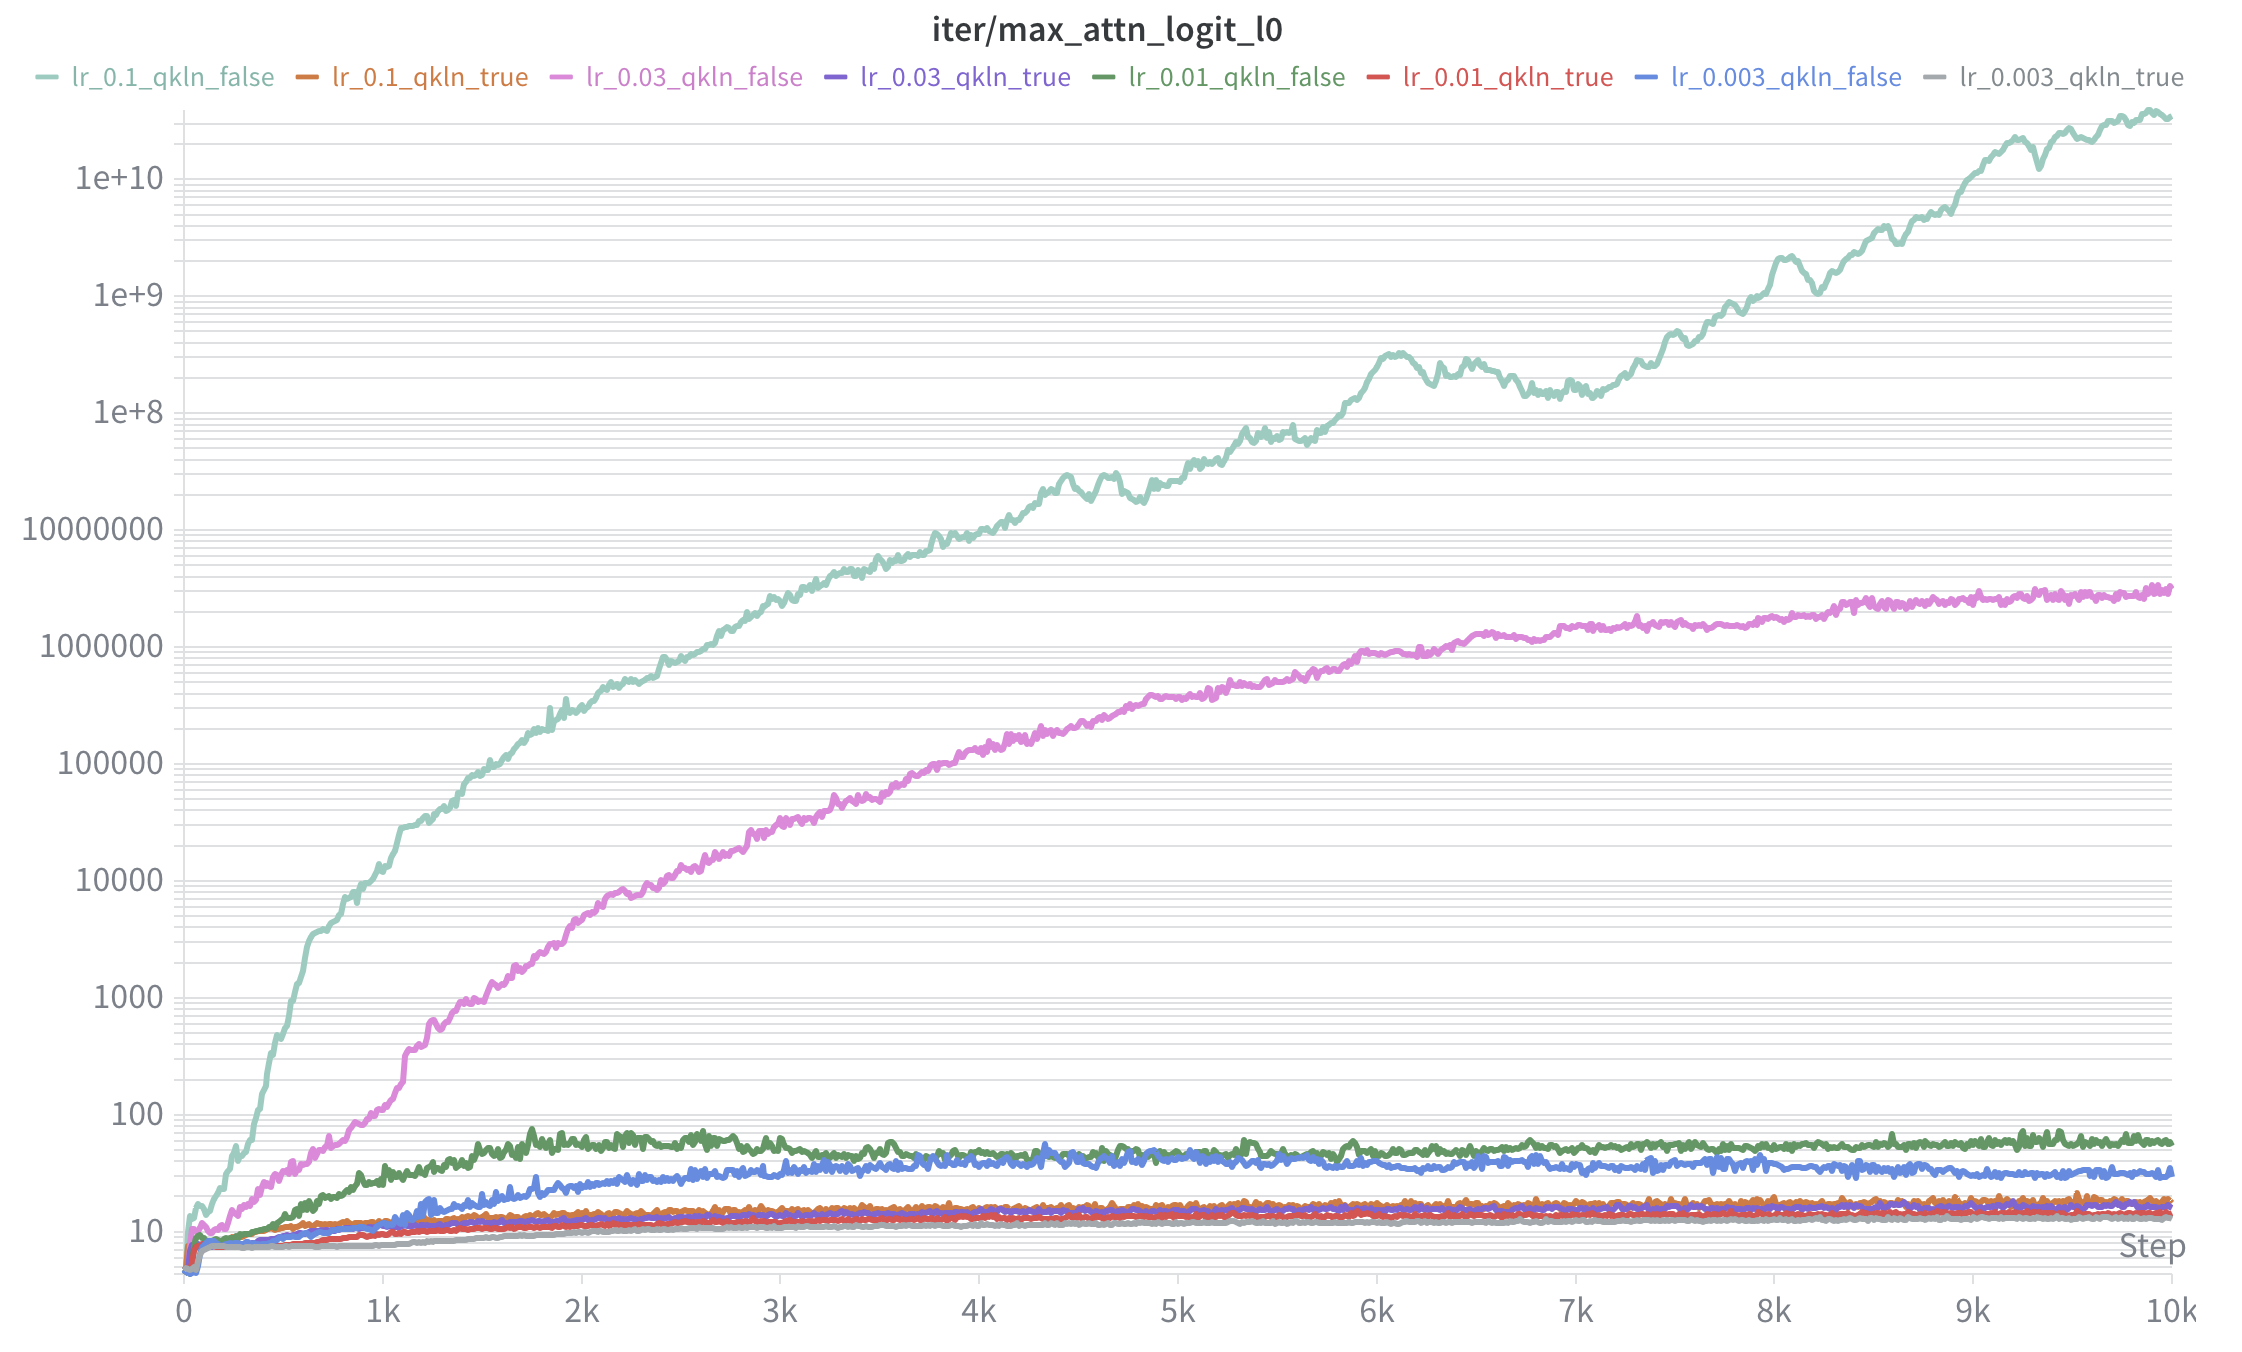
\includegraphics[width=0.7\linewidth]{figures/C1_max_attn_logits.png}
    \caption{Evolution of the maximum attention logits in the first layer. Divergence occurs at high learning rates when qk-layernorm is not used.}
\end{figure}
We observe that attention logits diverge when: $\eta \geq 0.03 \quad \text{and qk-layernorm is disabled}$. And this behavior is consistent with their findings. We then report the following learning rate sensitivy : \textbf{0.025} with qk-layernorm and \textbf{1.37} without, and  (unfortunately it is not a curve depending, only for a given parameters size, here $\approx$50M), which follows their results. 



\paragraph{Origin of the Instability: Norm Explosion} To confirm the origin of this divergence, we track the mean norms of queries and keys, and observe that the norms of $Q$ and $K$ increase rapidly, reproducing the results proposed in appendix of the paper. 
\begin{figure}[H]
\centering
\begin{subfigure}{0.48\linewidth}
    \centering
    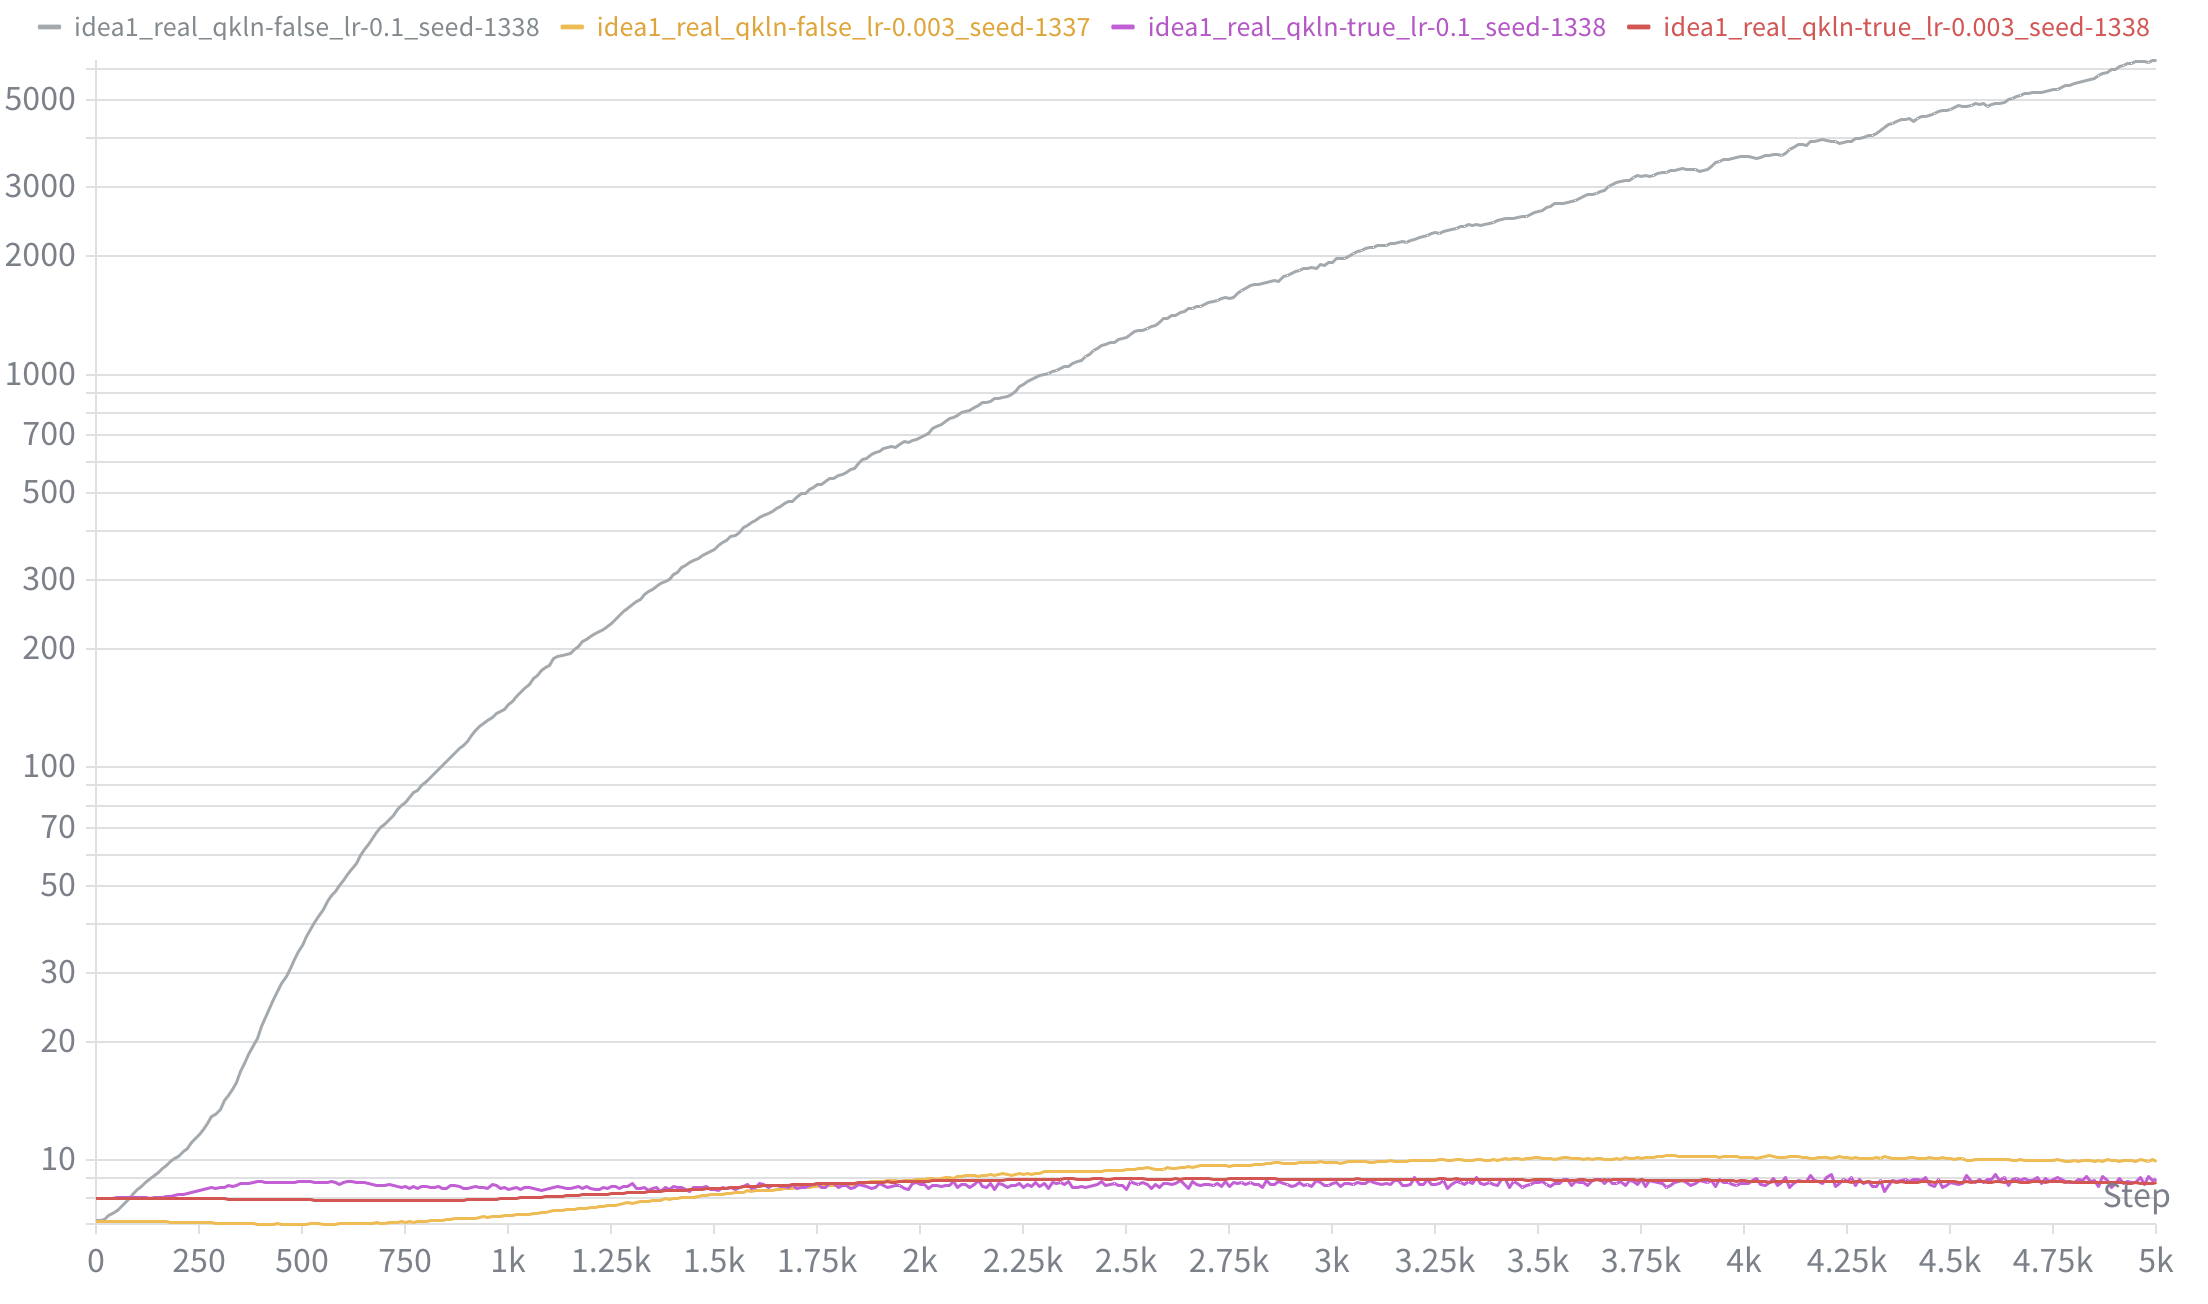
\includegraphics[width=\linewidth]{figures/C1_qnorm.png}
    \caption{Mean norm of $Q$}
\end{subfigure}
\hfill
\begin{subfigure}{0.48\linewidth}
    \centering
    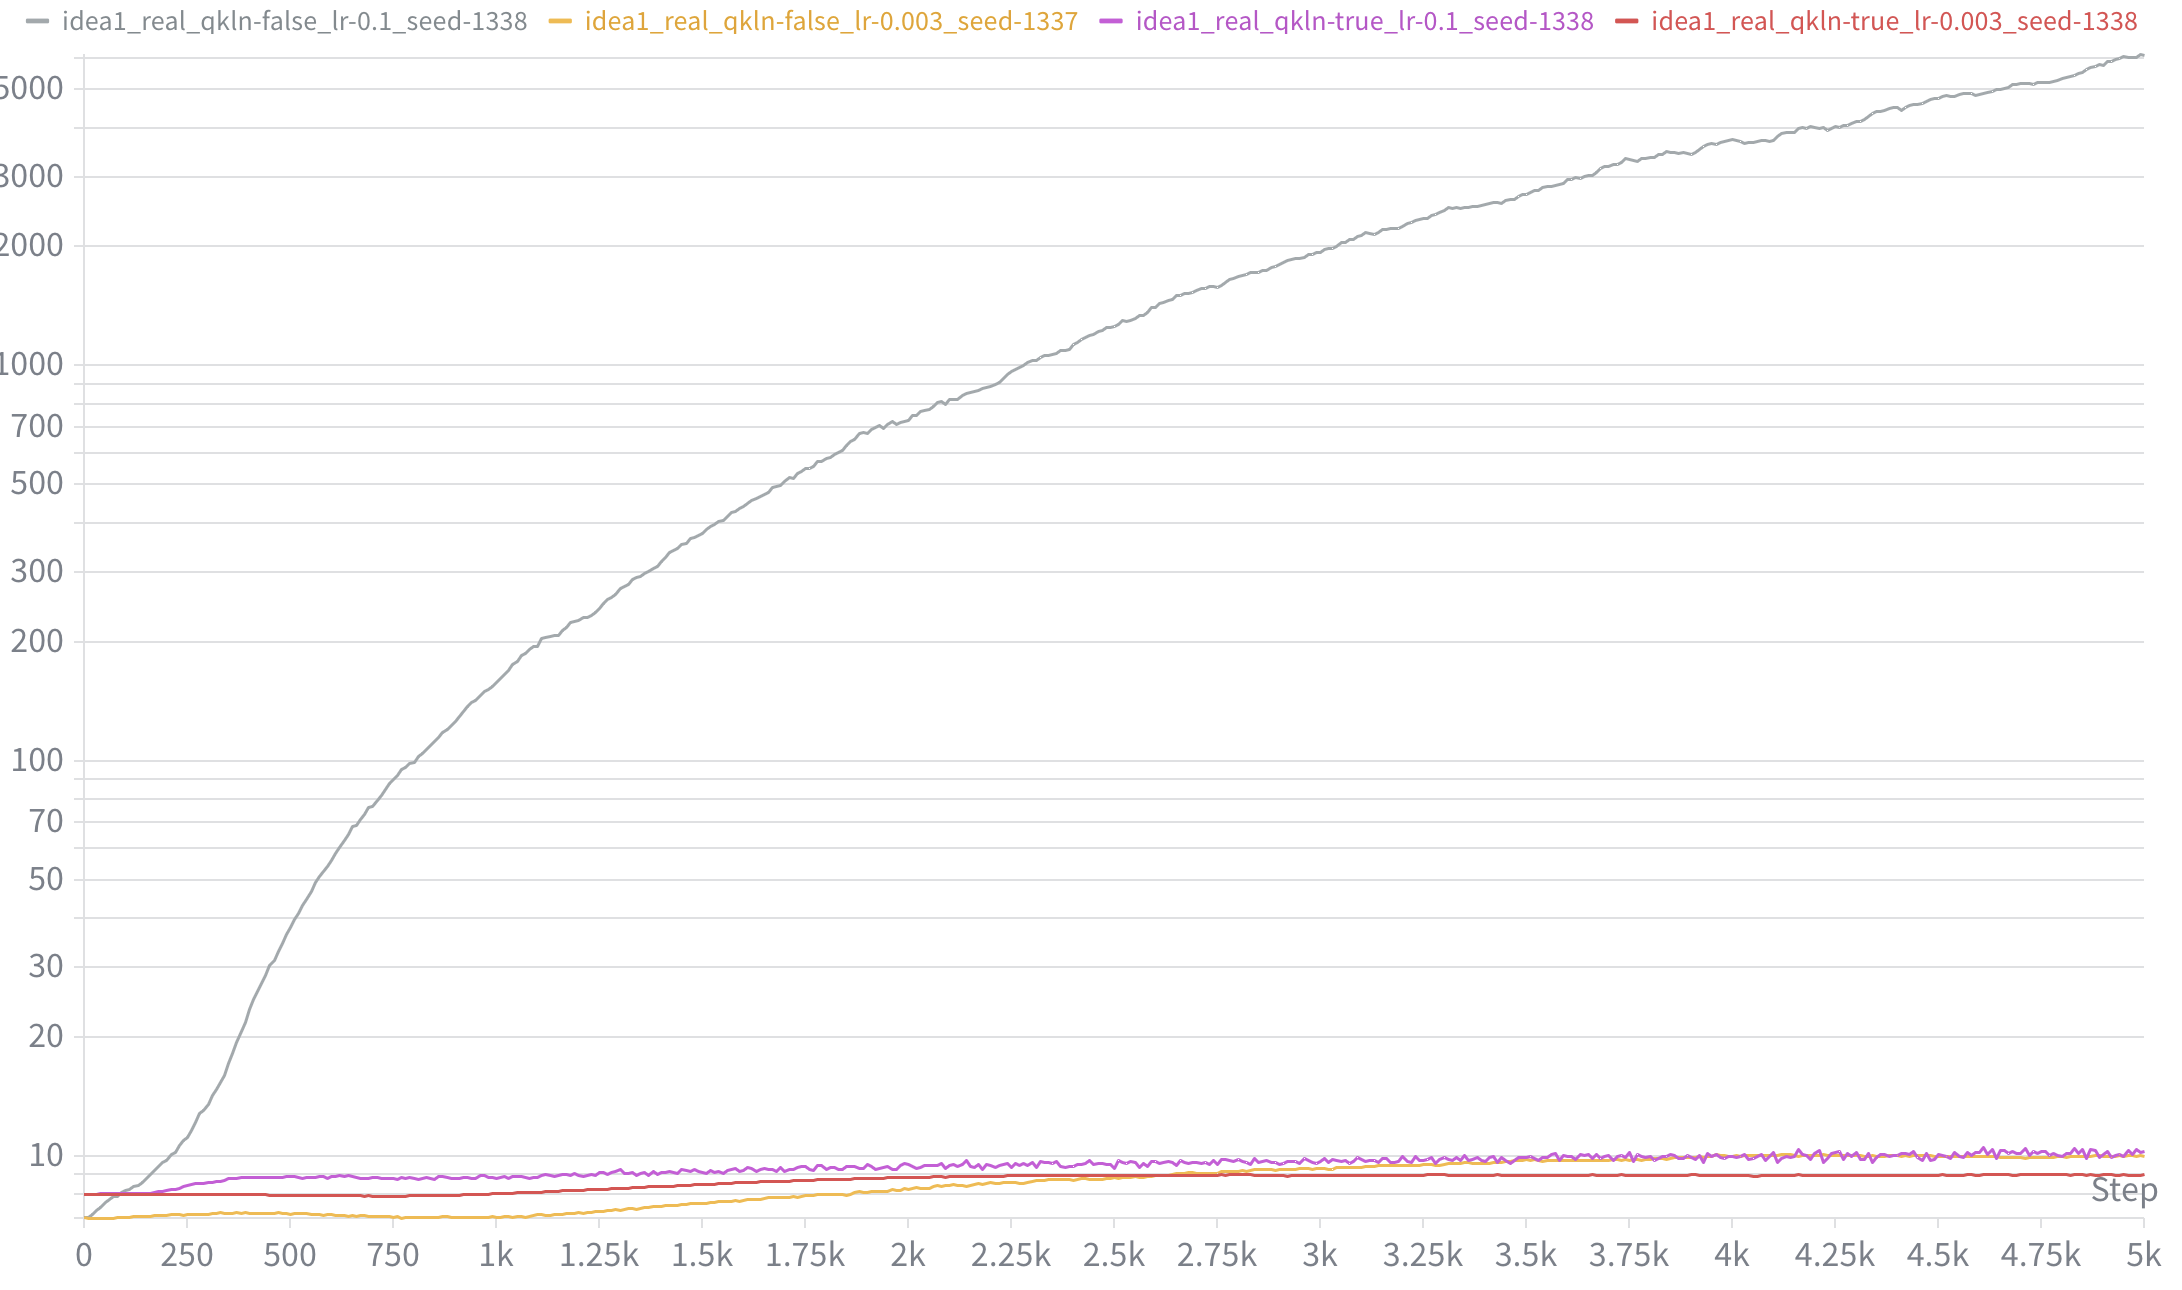
\includegraphics[width=\linewidth]{figures/C1_knorm.png}
    \caption{Mean norm of $K$}
\end{subfigure}
\caption{Evolution of query and key norms in the first attention layer.}
\end{figure}


\paragraph{Optimizer vs Data: Robustness Analysis}
In theory, for gradient descent, to avoid divergence, one requires with $\eta$ the learning rate : 
\[
\eta < \frac{2}{\lambda_{\max}(H)} \text{  and where $H$ is the Hessian of the loss: } H_{ij} = \frac{\partial^2 \mathcal{L}}{\partial \theta_i \partial \theta_j}
\]
This quantity is too large to compute in practice, but can be approximated. Moreover, $H$ depends on the parameters, but also on the training process and therefore on the data $\mathcal{D}$ : $H = H(\theta_{\text{step}}, \mathcal{D})$
where the dynamic is included in $\theta_{\text{step}}$ (as noted by the authors, the curvature varies during training). The \textit{data-driven} aspect can be interpreted as defining the global loss landscape, while the \textit{optimization-driven} aspect determines where we are located in this landscape and how we evolve within it.

The original work suggests that this instability is optimizer-driven rather than data-dependent. We validate this hypothesis by comparing different dataset constructions. A dataset is said to be IID (independent and identically distributed) if: $x_1, x_2, \dots, x_n \sim \mathcal{D}$ where all samples are independent and drawn from the same distribution. In practice, this removes any sequential or structural dependencies. A shuffled dataset consists of the same samples but randomly permuted. Unlike IID data, local dependencies may still exist, but global ordering is destroyed. 

\begin{figure}[H]
\centering
\begin{subfigure}{0.48\linewidth}
    \centering
    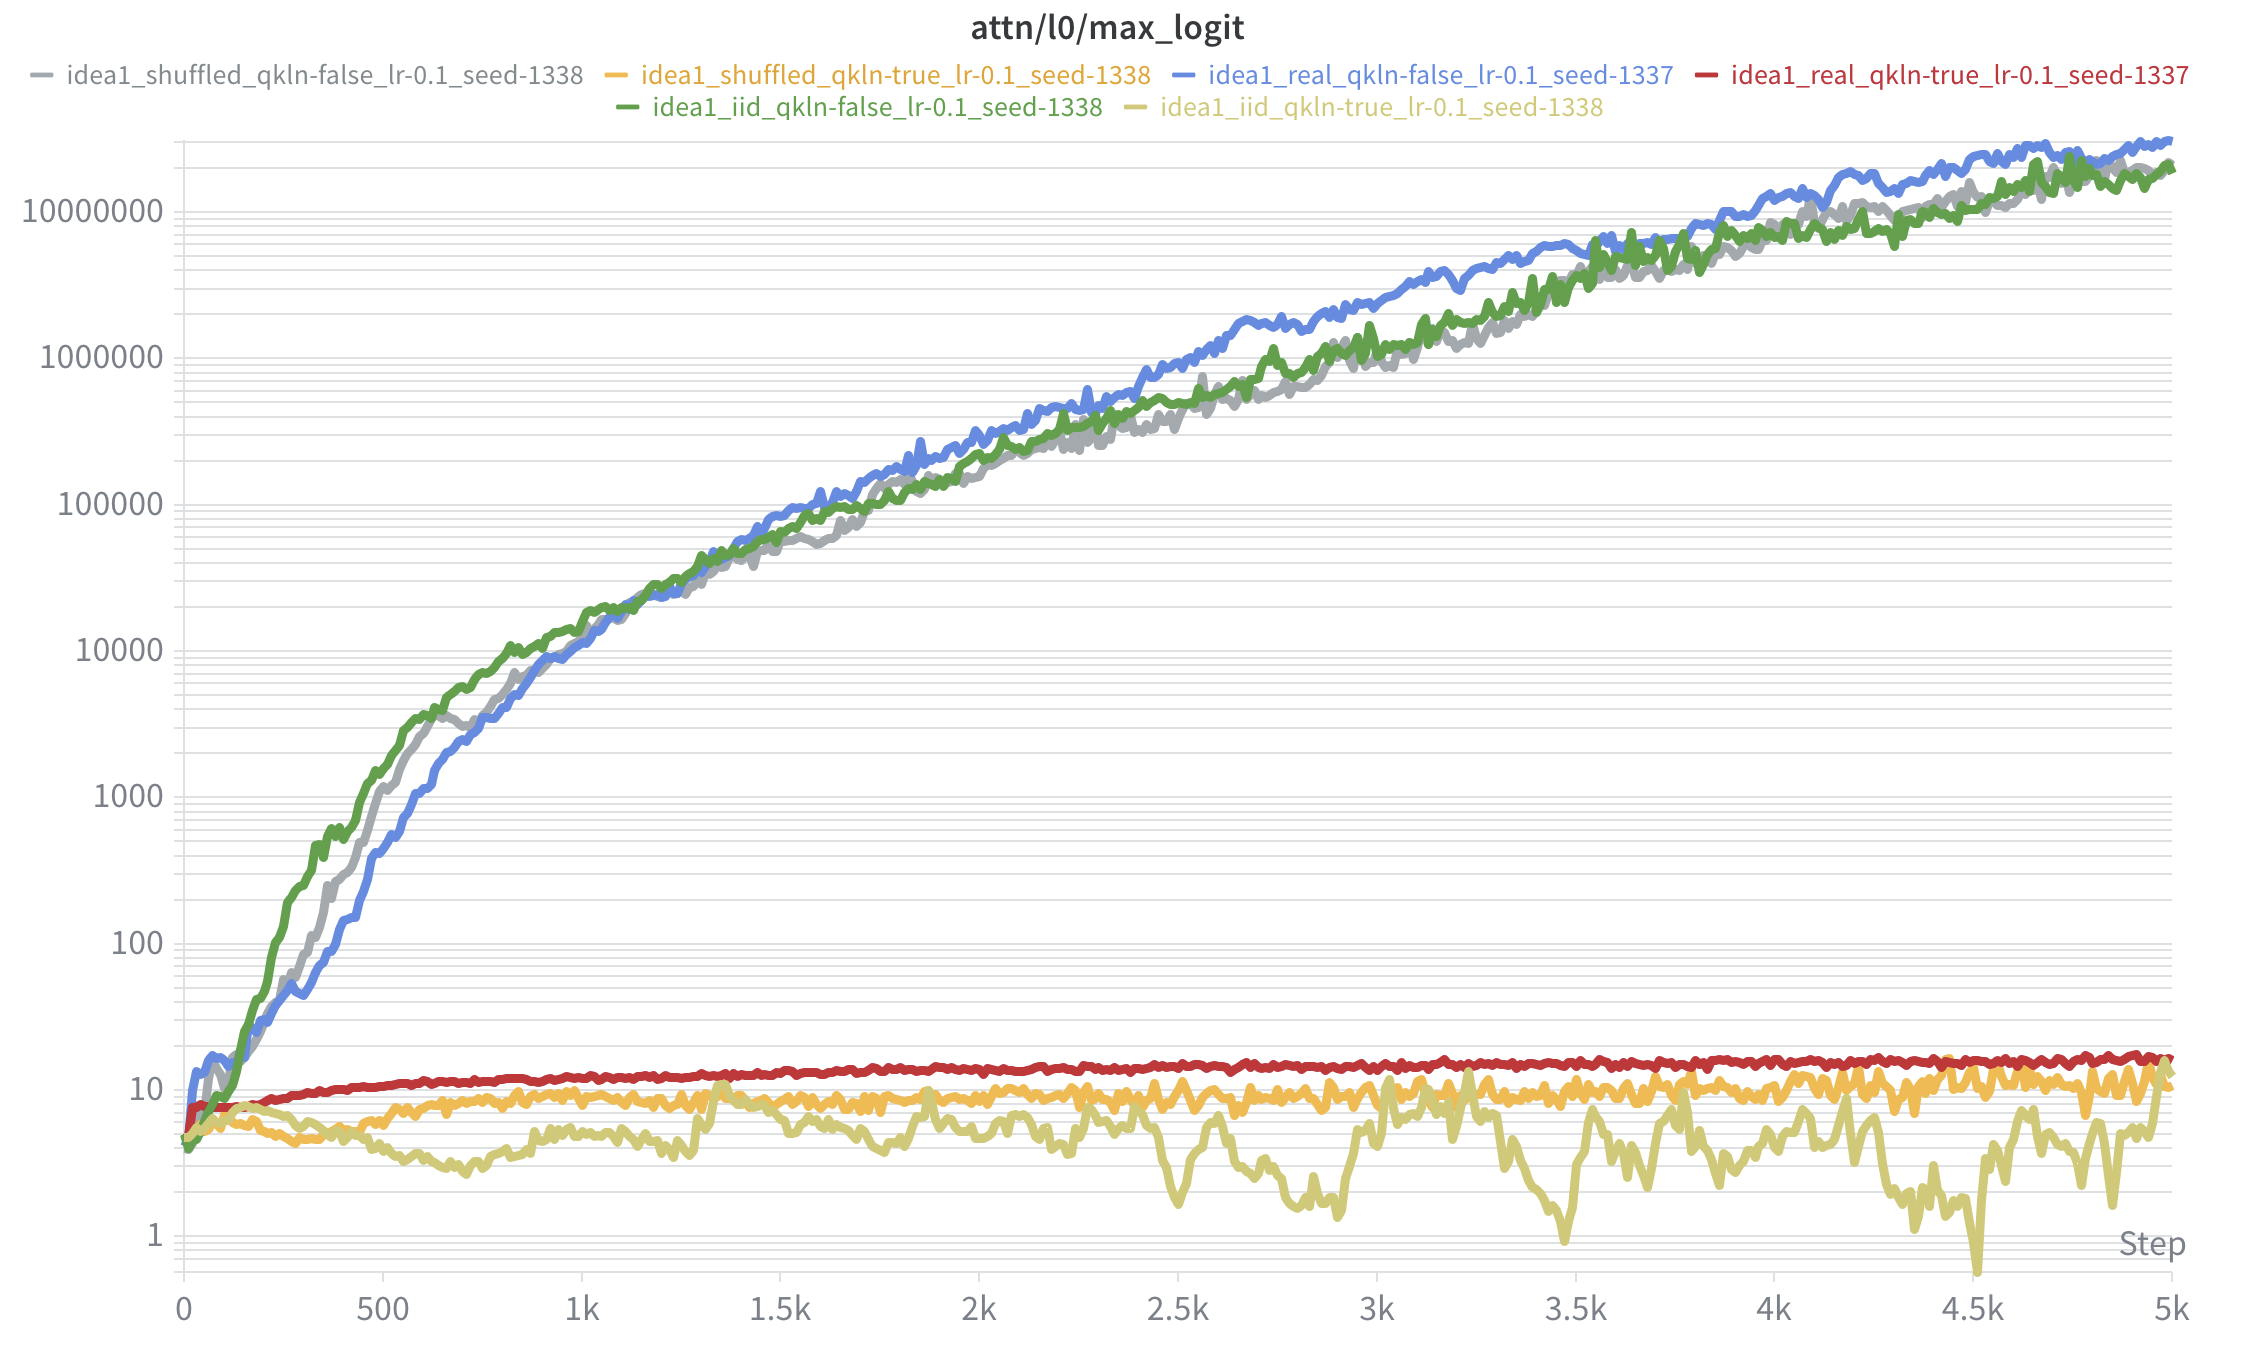
\includegraphics[width=\linewidth]{figures/C1_multiple_data.png}
    \caption{Maximum attention logits}
\end{subfigure}
\hfill
\begin{subfigure}{0.48\linewidth}
    \centering
    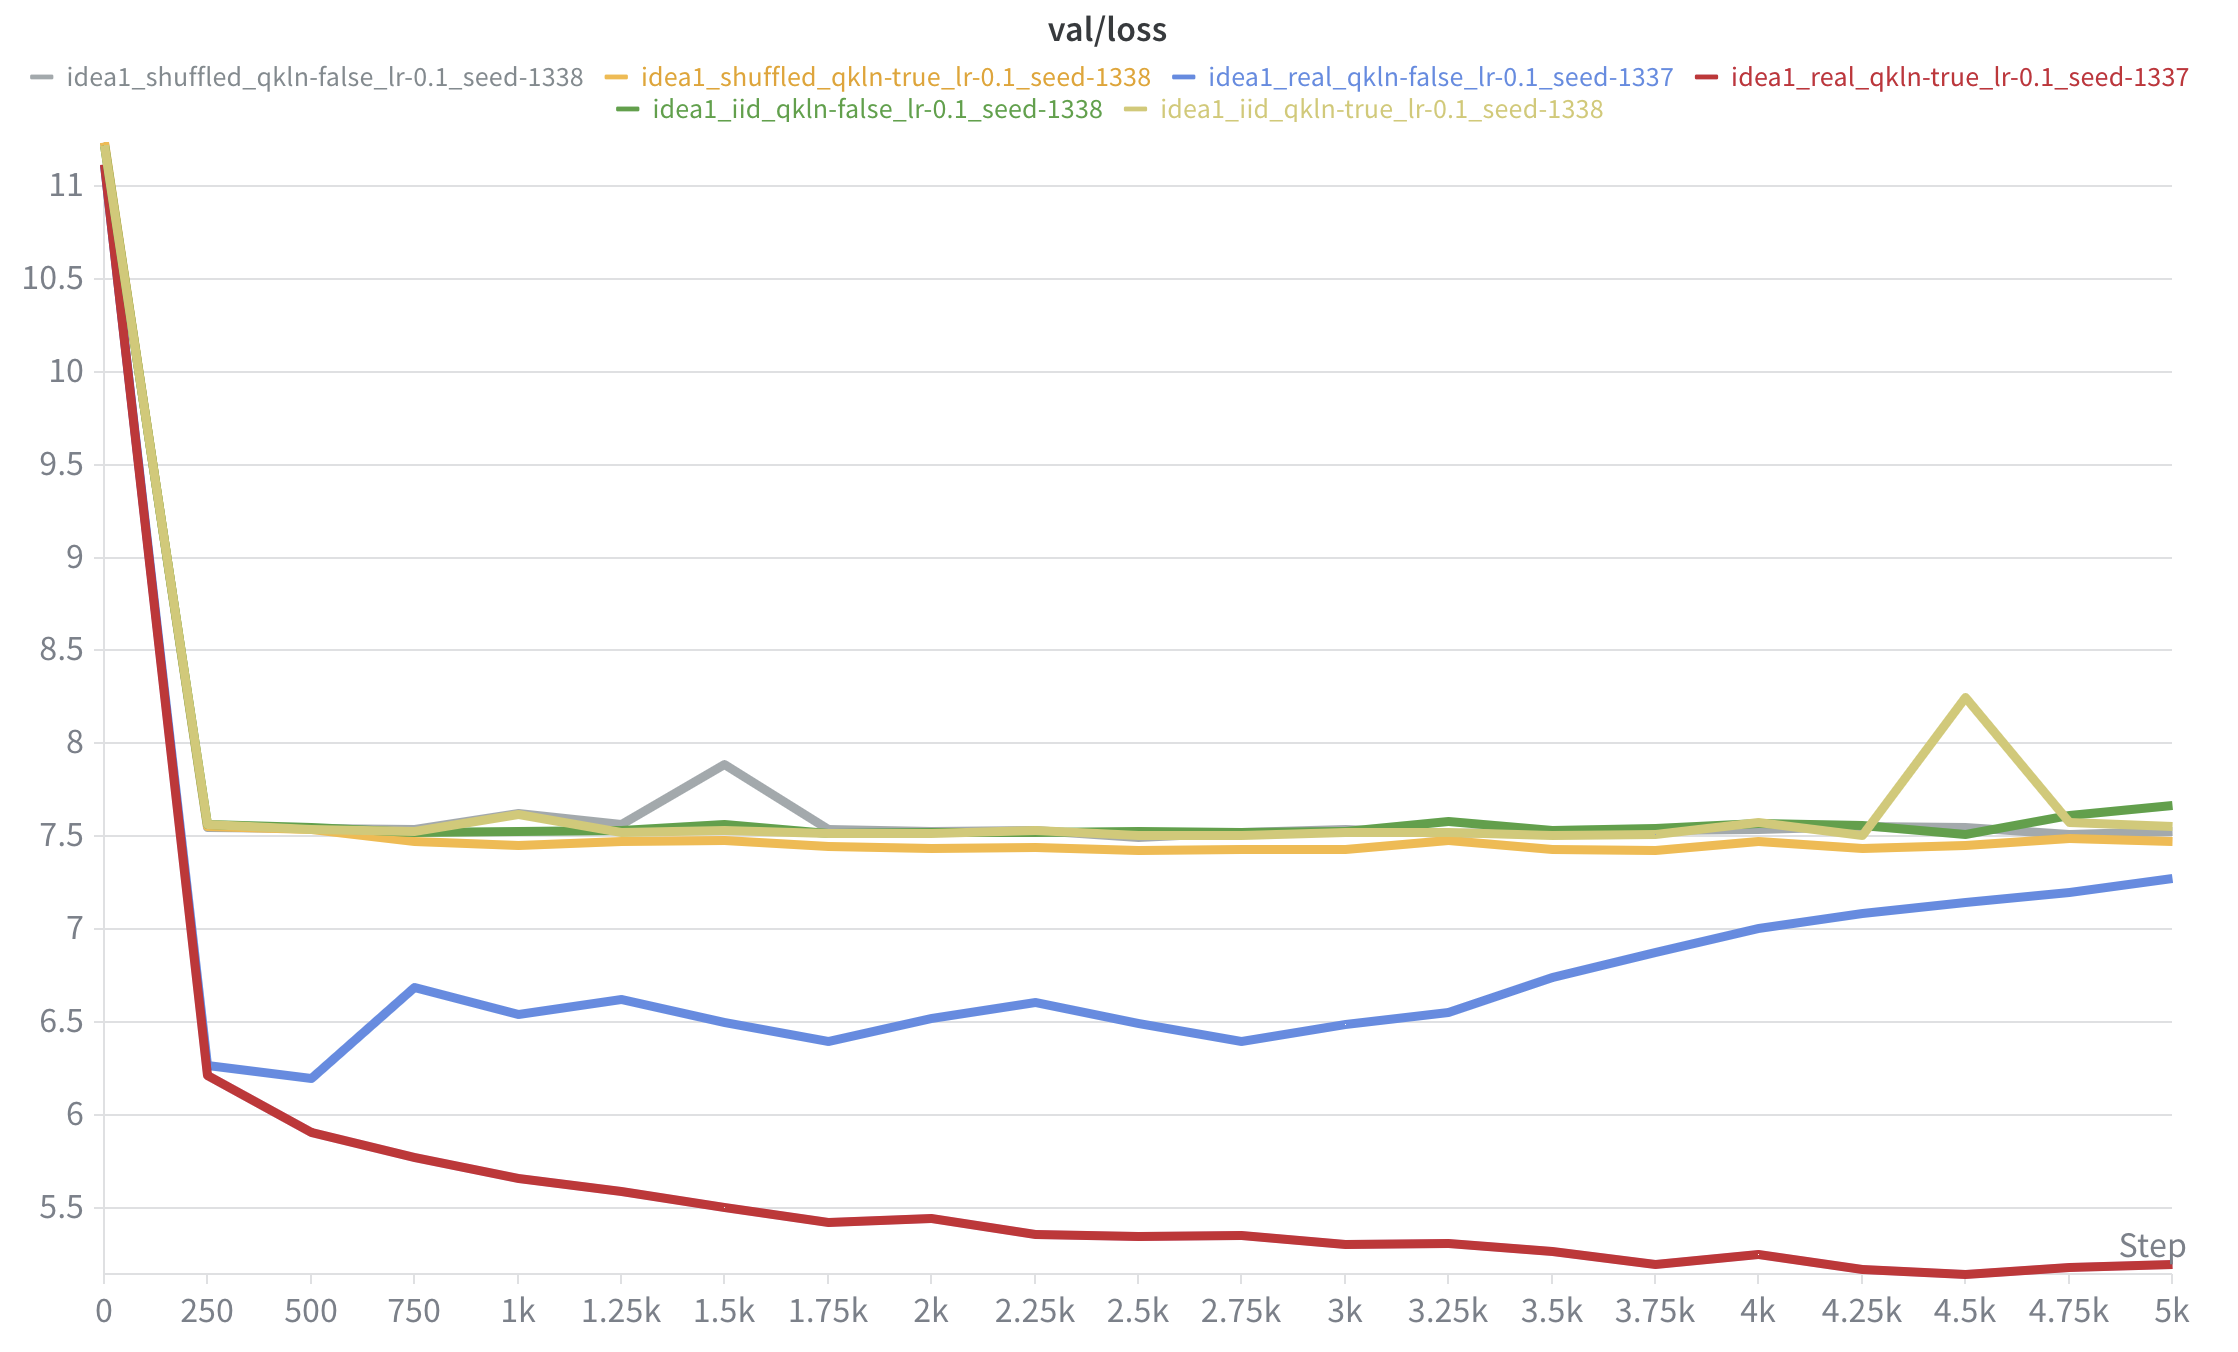
\includegraphics[width=\linewidth]{figures/C1_losses_datasets.png}
    \caption{Validation loss}
\end{subfigure}
\caption{Comparison across standard, shuffled, and IID datasets. Note that for iid and shuffled it is higher as the model can only overfit the training data without learning to generalize.}
\end{figure}
As we observe that logit divergence occurs in all settings, our experiments confirm that instabilities are more driven by the dynamics:
\[
\text{stability} \sim \frac{\eta}{\lambda_{\max}(H(\theta_{\text{step}}, \mathcal{D}))}
\approx \frac{\eta}{\lambda_{\max}(H(\theta_{\text{step}}))}.
\]




\subsection{Claim 2}

Our reproduction of Claim~2 was ultimately unsuccessful.
While the paper reports a clear output-logit divergence when weight decay is
removed, we did not observe the same phenomenon reliably in our small-scale
setting.
Across the runs we carried out, the mean output logit either remained
comparatively well-behaved, or training became unstable in a more global and
less interpretable way before any clean divergence pattern emerged.

To make the instability easier to trigger, we deliberately explored more
aggressive training settings than our default setup.
In particular, we disabled gradient clipping, increased the learning rate,
removed learning-rate warmup, and disabled learning-rate decay.
These changes were intended to stress the optimisation dynamics and reproduce
the failure mode described in the paper more quickly.
However, this did not lead to a convincing confirmation of the claim.

Instead, we observed two broad outcomes.
In some runs, training remained stable enough that the output logit mean did
not exhibit the expected runaway behaviour, even in the no-weight-decay
configuration.
In other runs, optimisation became unstable more abruptly, with large training
pathologies that made the behaviour difficult to attribute specifically to the
output-logit mechanism discussed by~\citet{wortsman2023smallscale}.
As a result, our experiments do not provide clear evidence that removing weight
decay alone causes the output logit mean to explode in our setting, nor do they
allow us to cleanly isolate the stabilising effect of z-loss.

We nevertheless report representative figures from these runs.
They illustrate the main outcome of our reproduction attempt: depending on the
configuration, we observed either no clear divergence in the output logit mean
or severe overall optimisation instability, but not the clean qualitative
pattern described in the original paper.

\begin{figure}[H]
    \centering

    % -------- Row 1: Stable --------
    \begin{subfigure}{0.48\textwidth}
        \centering
        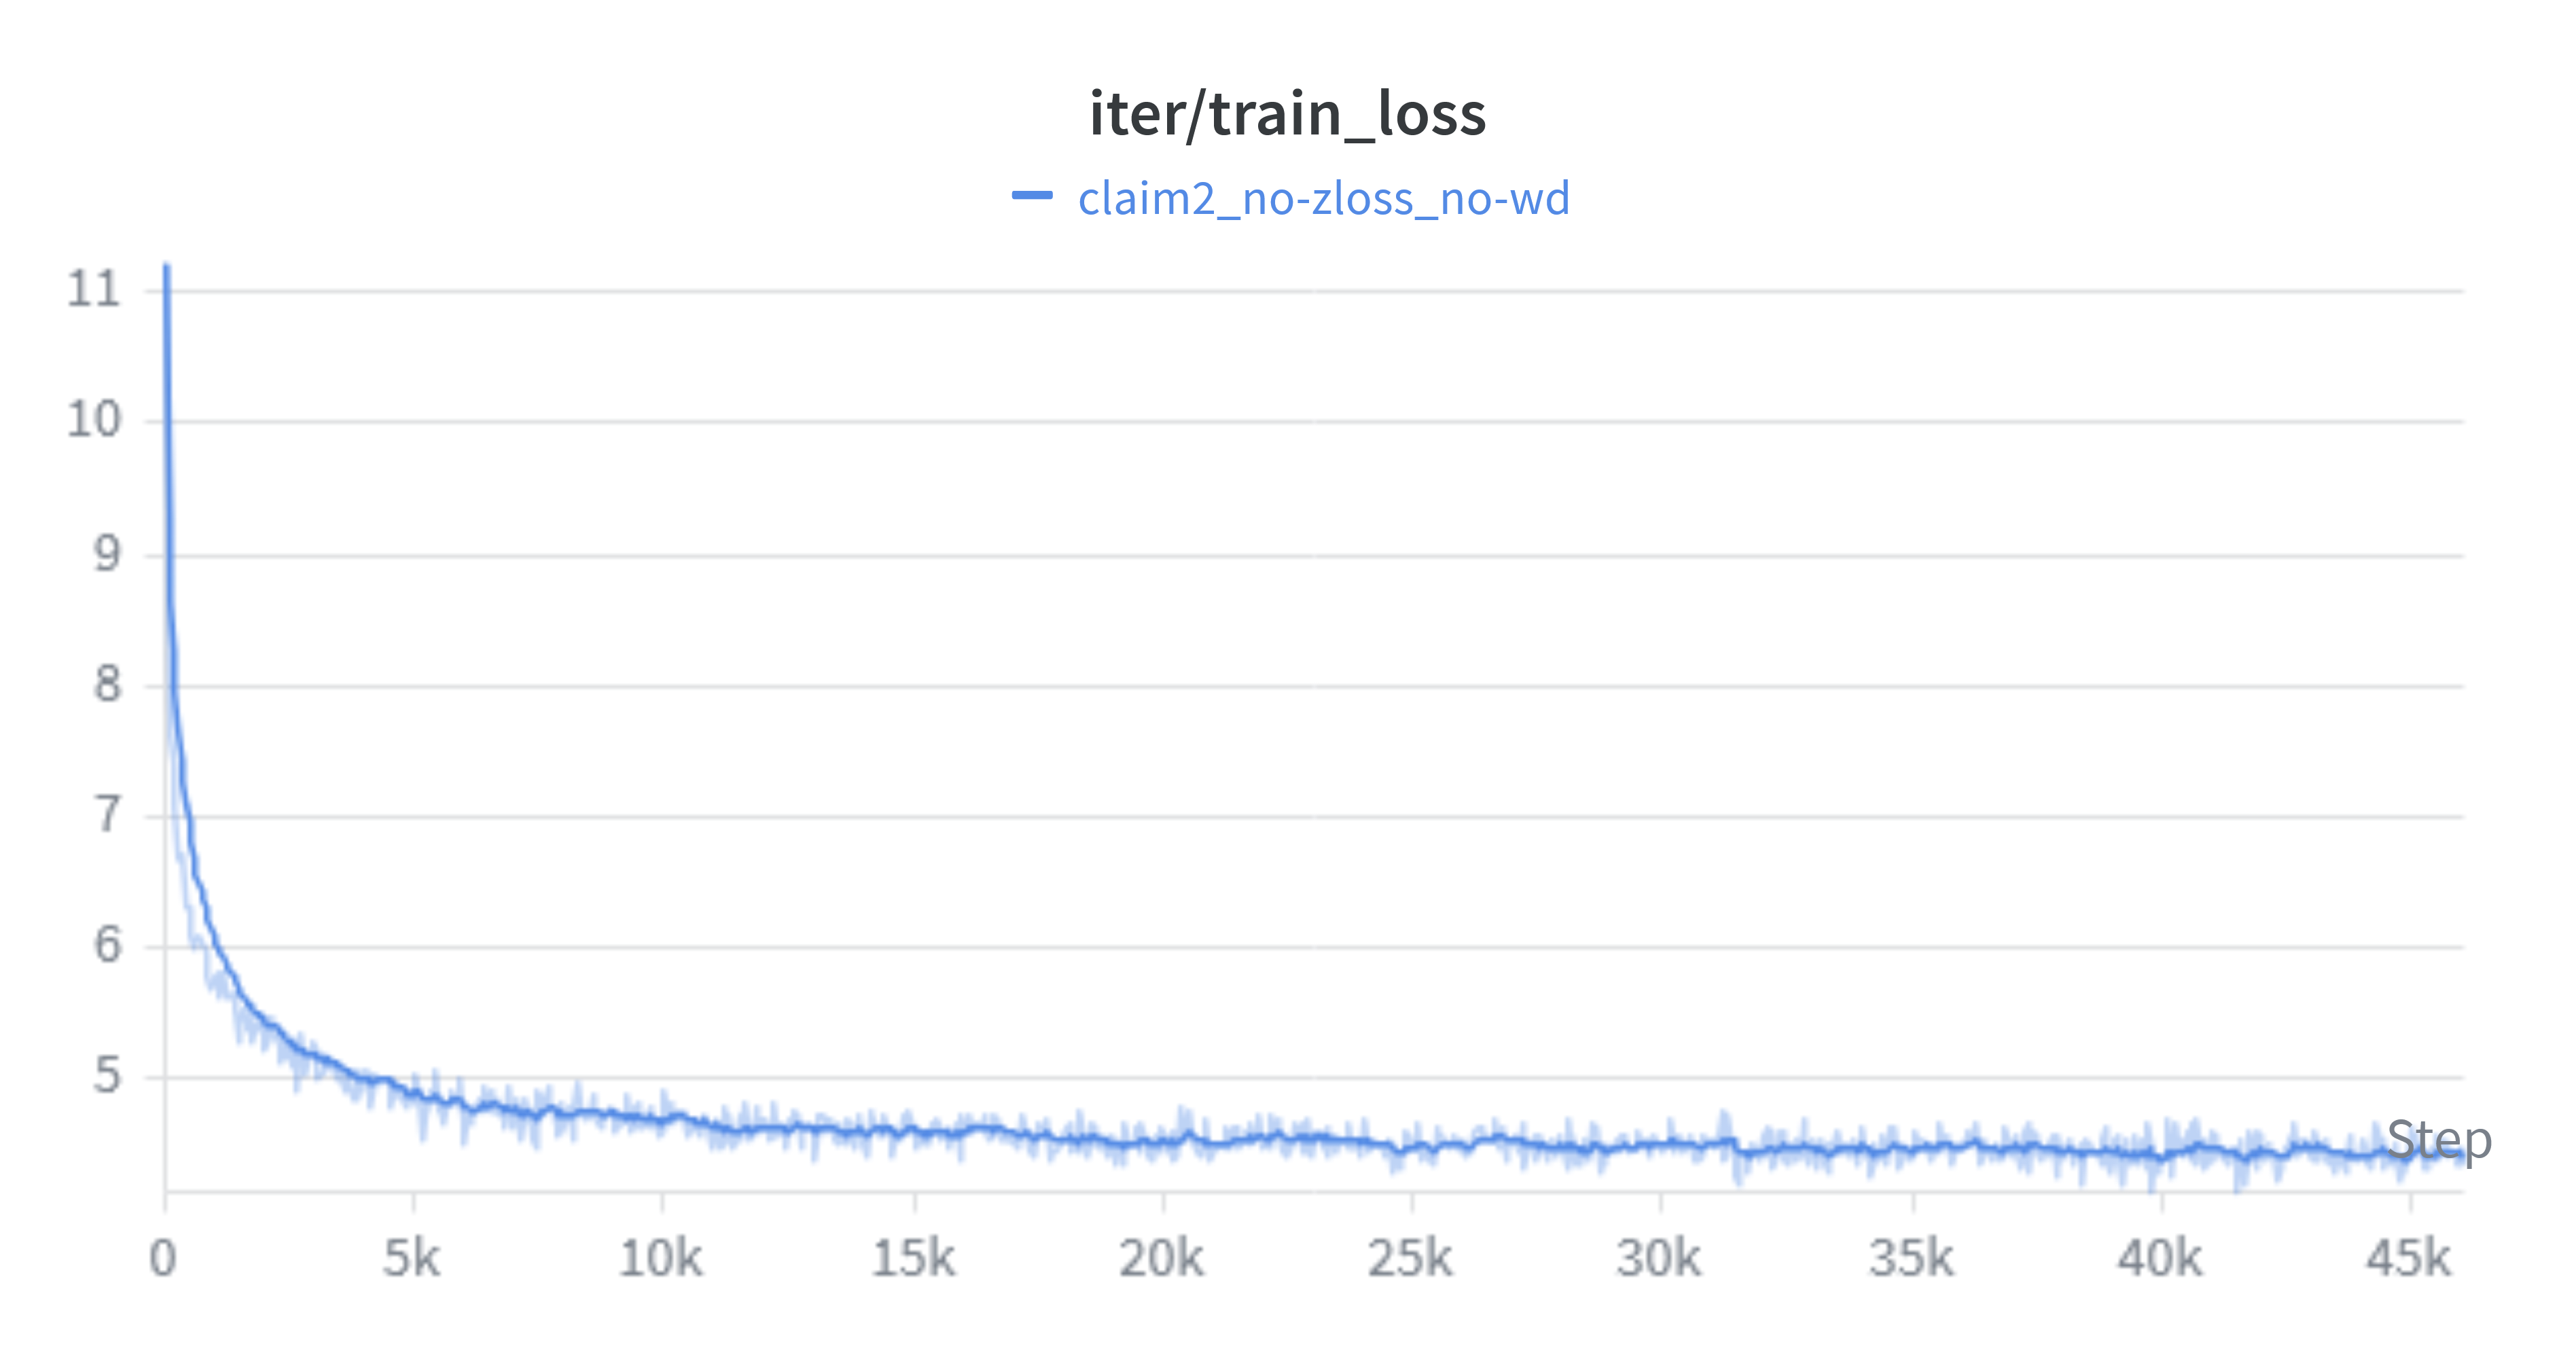
\includegraphics[width=\linewidth]{figures/C2_train_loss_stable.png}
        \caption{Stable — train loss}
    \end{subfigure}
    \hfill
    \begin{subfigure}{0.48\textwidth}
        \centering
        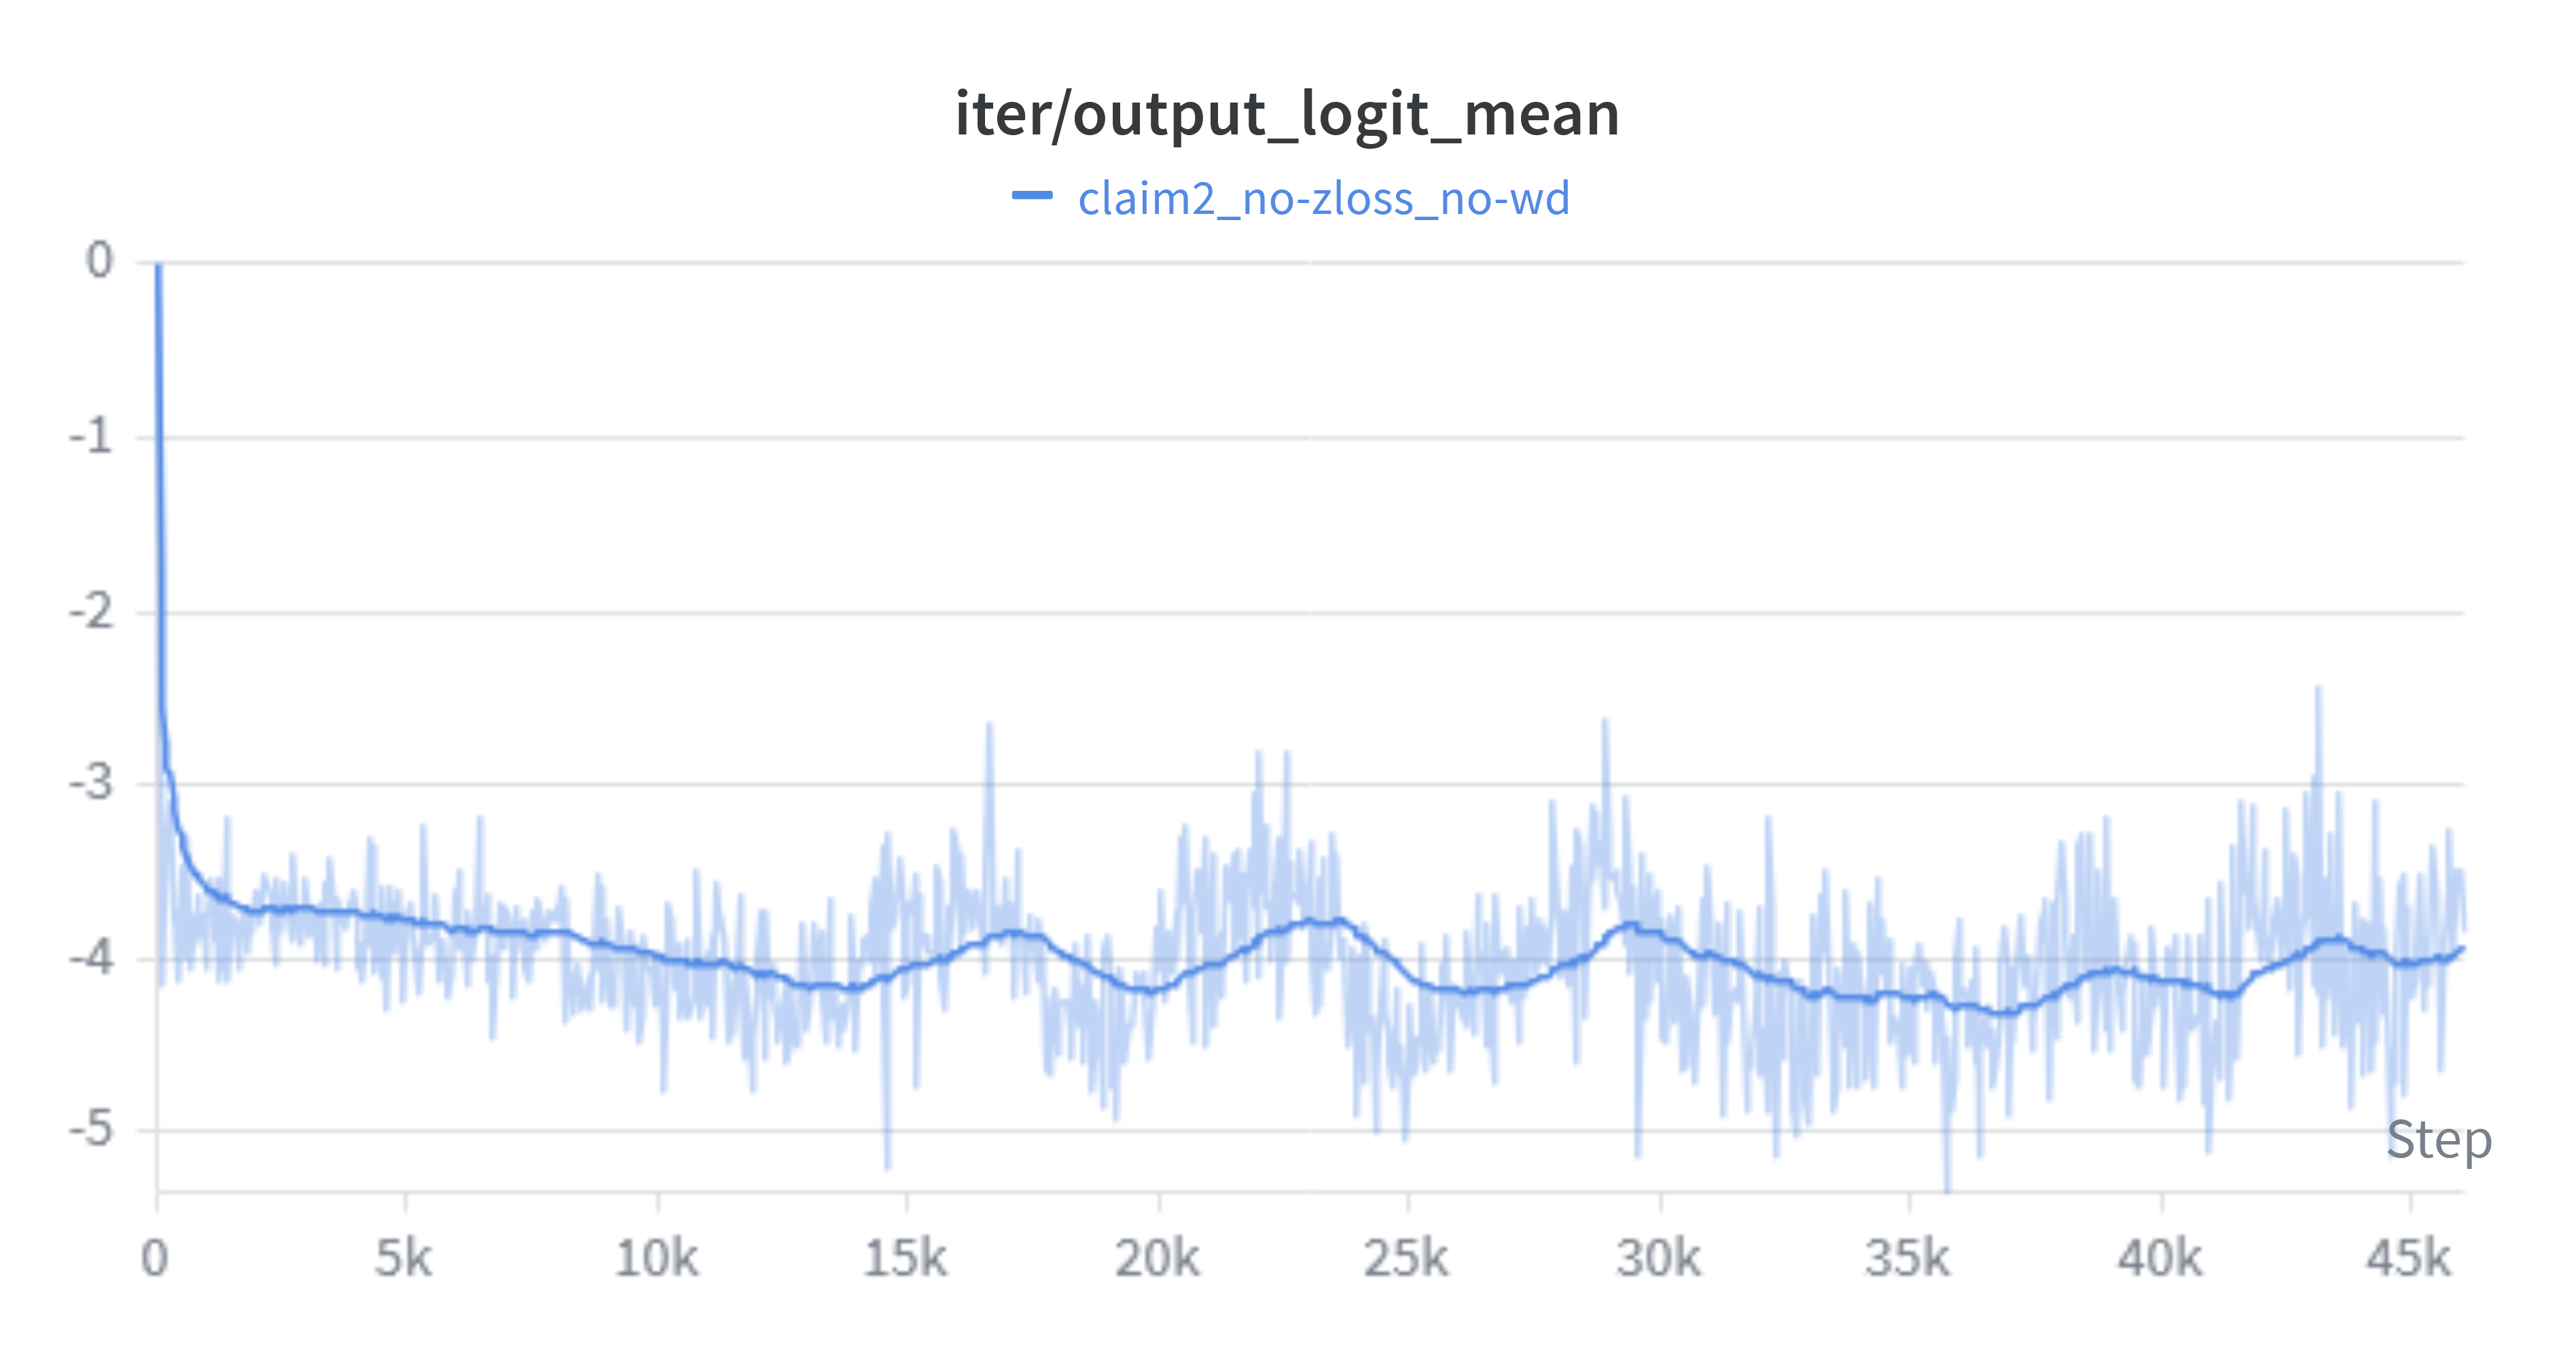
\includegraphics[width=\linewidth]{figures/C2_logit_mean_stable.png}
        \caption{Stable — logit mean}
    \end{subfigure}

    \vspace{0.5em}

    % -------- Row 2: OK stable --------
    \begin{subfigure}{0.48\textwidth}
        \centering
        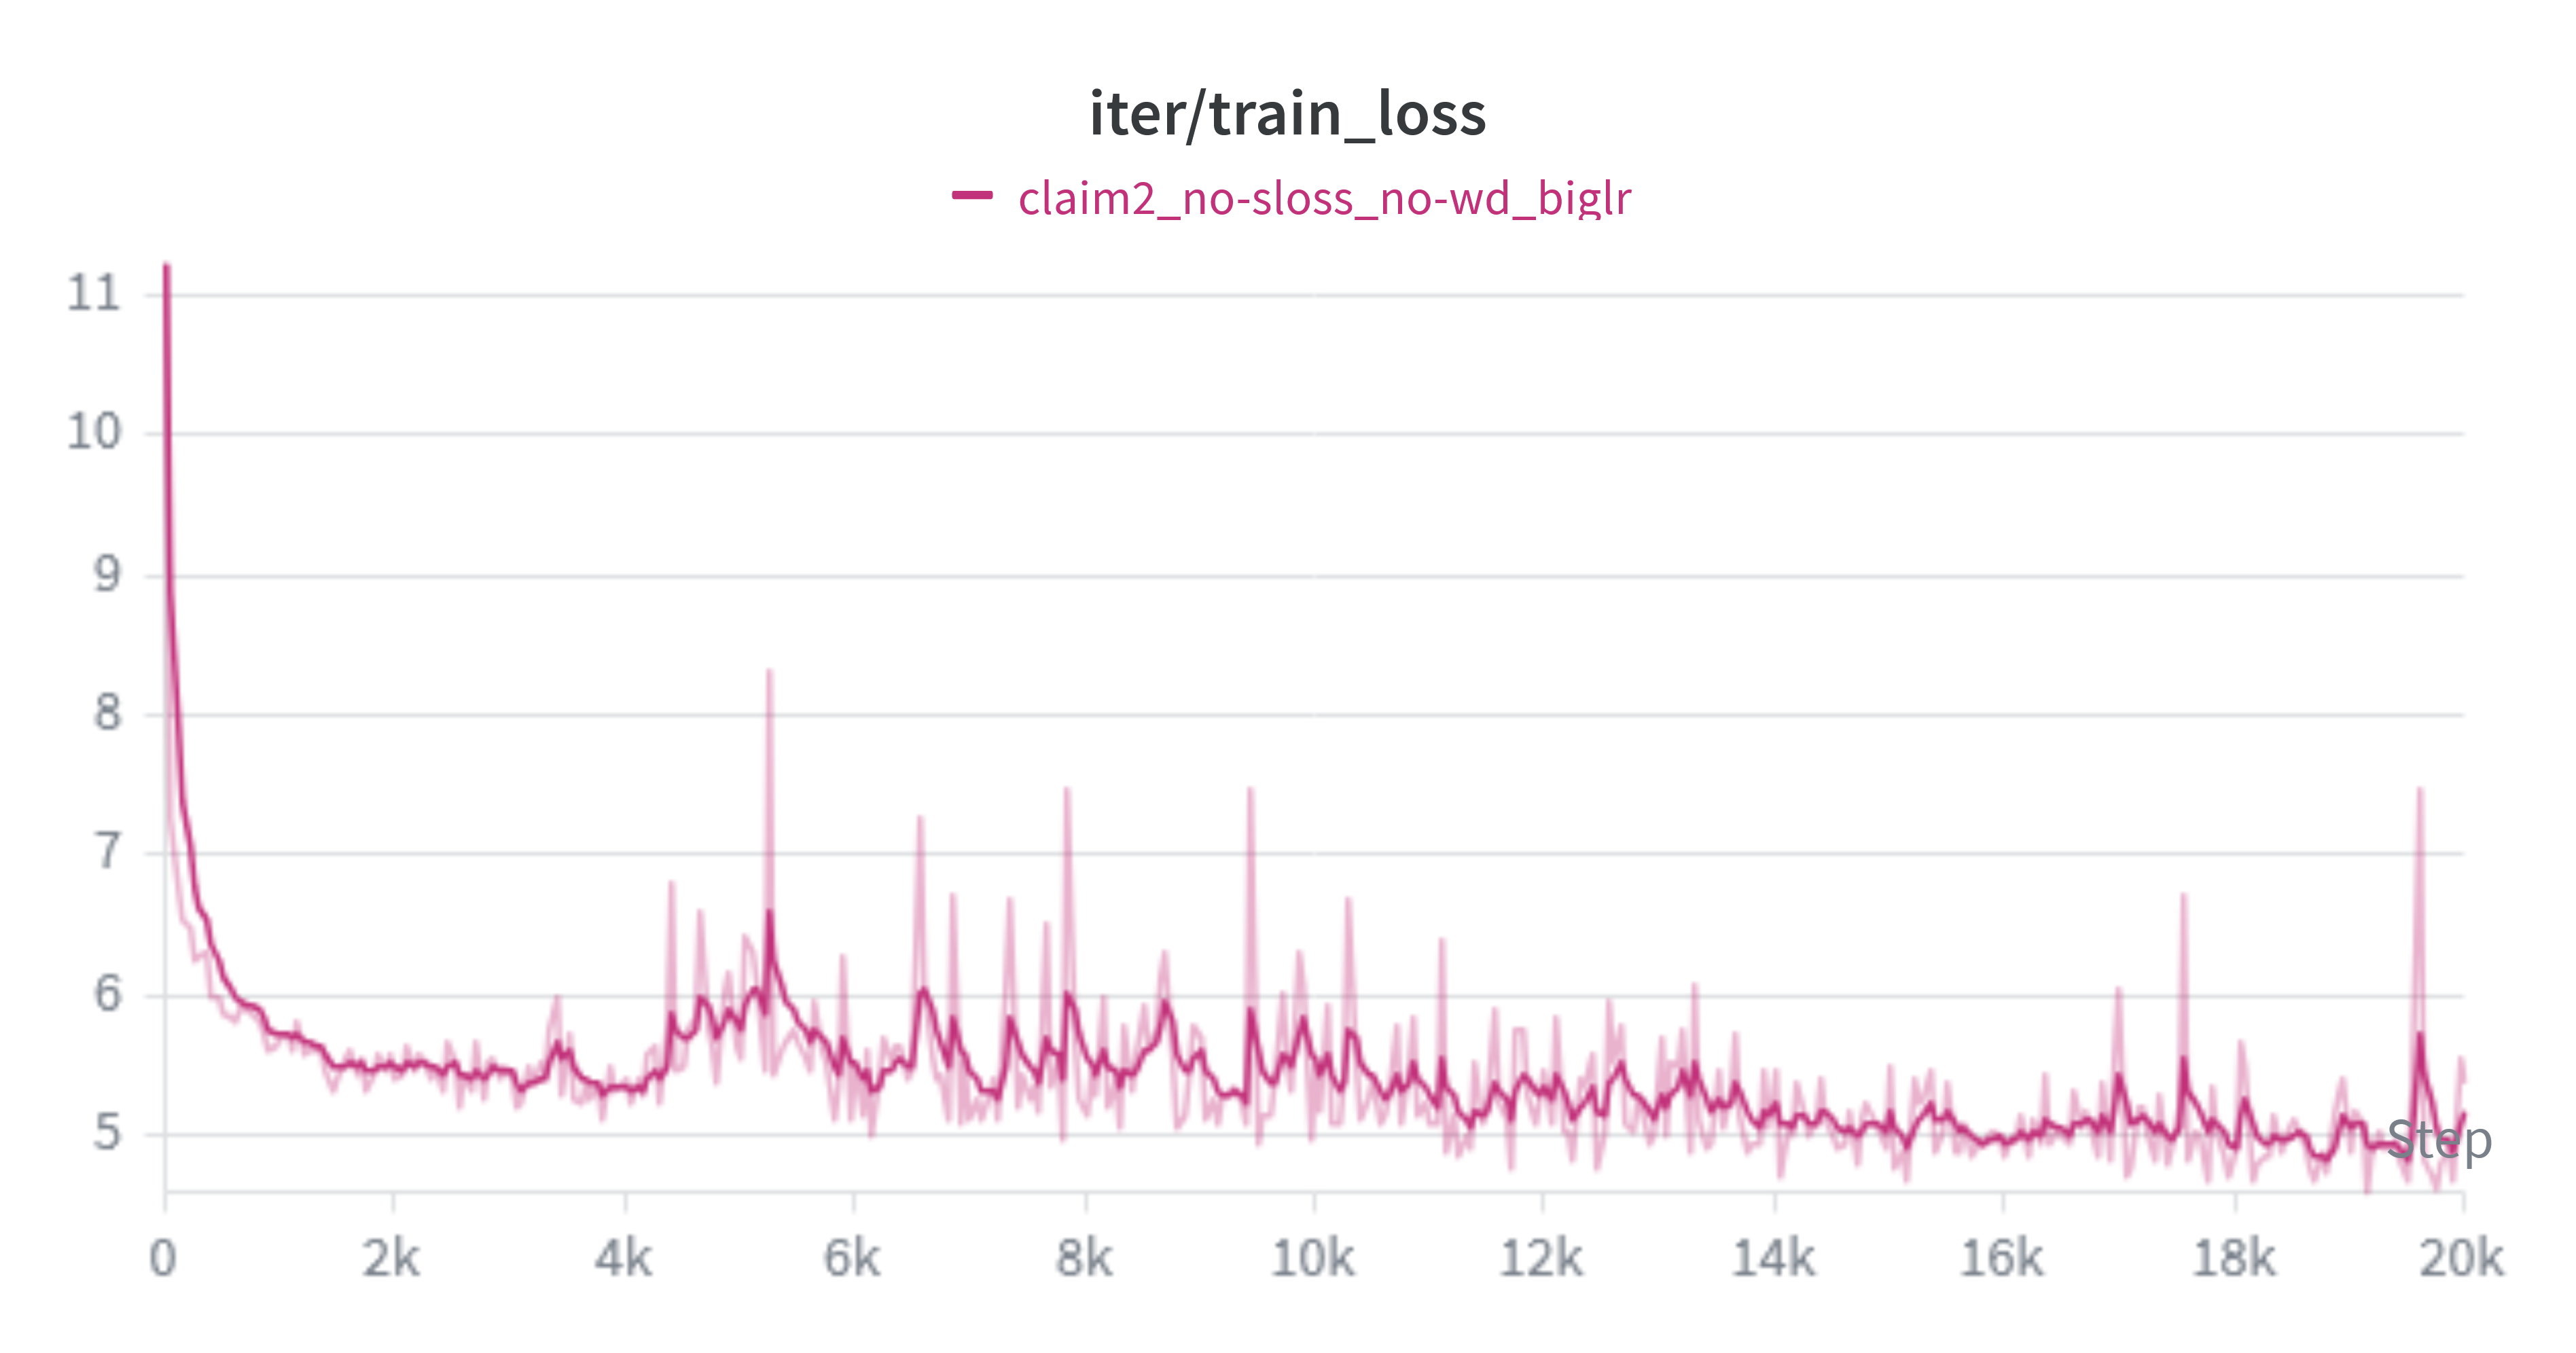
\includegraphics[width=\linewidth]{figures/C2_train_loss_mehstable.png}
        \caption{Moderately stable — train loss}
    \end{subfigure}
    \hfill
    \begin{subfigure}{0.48\textwidth}
        \centering
        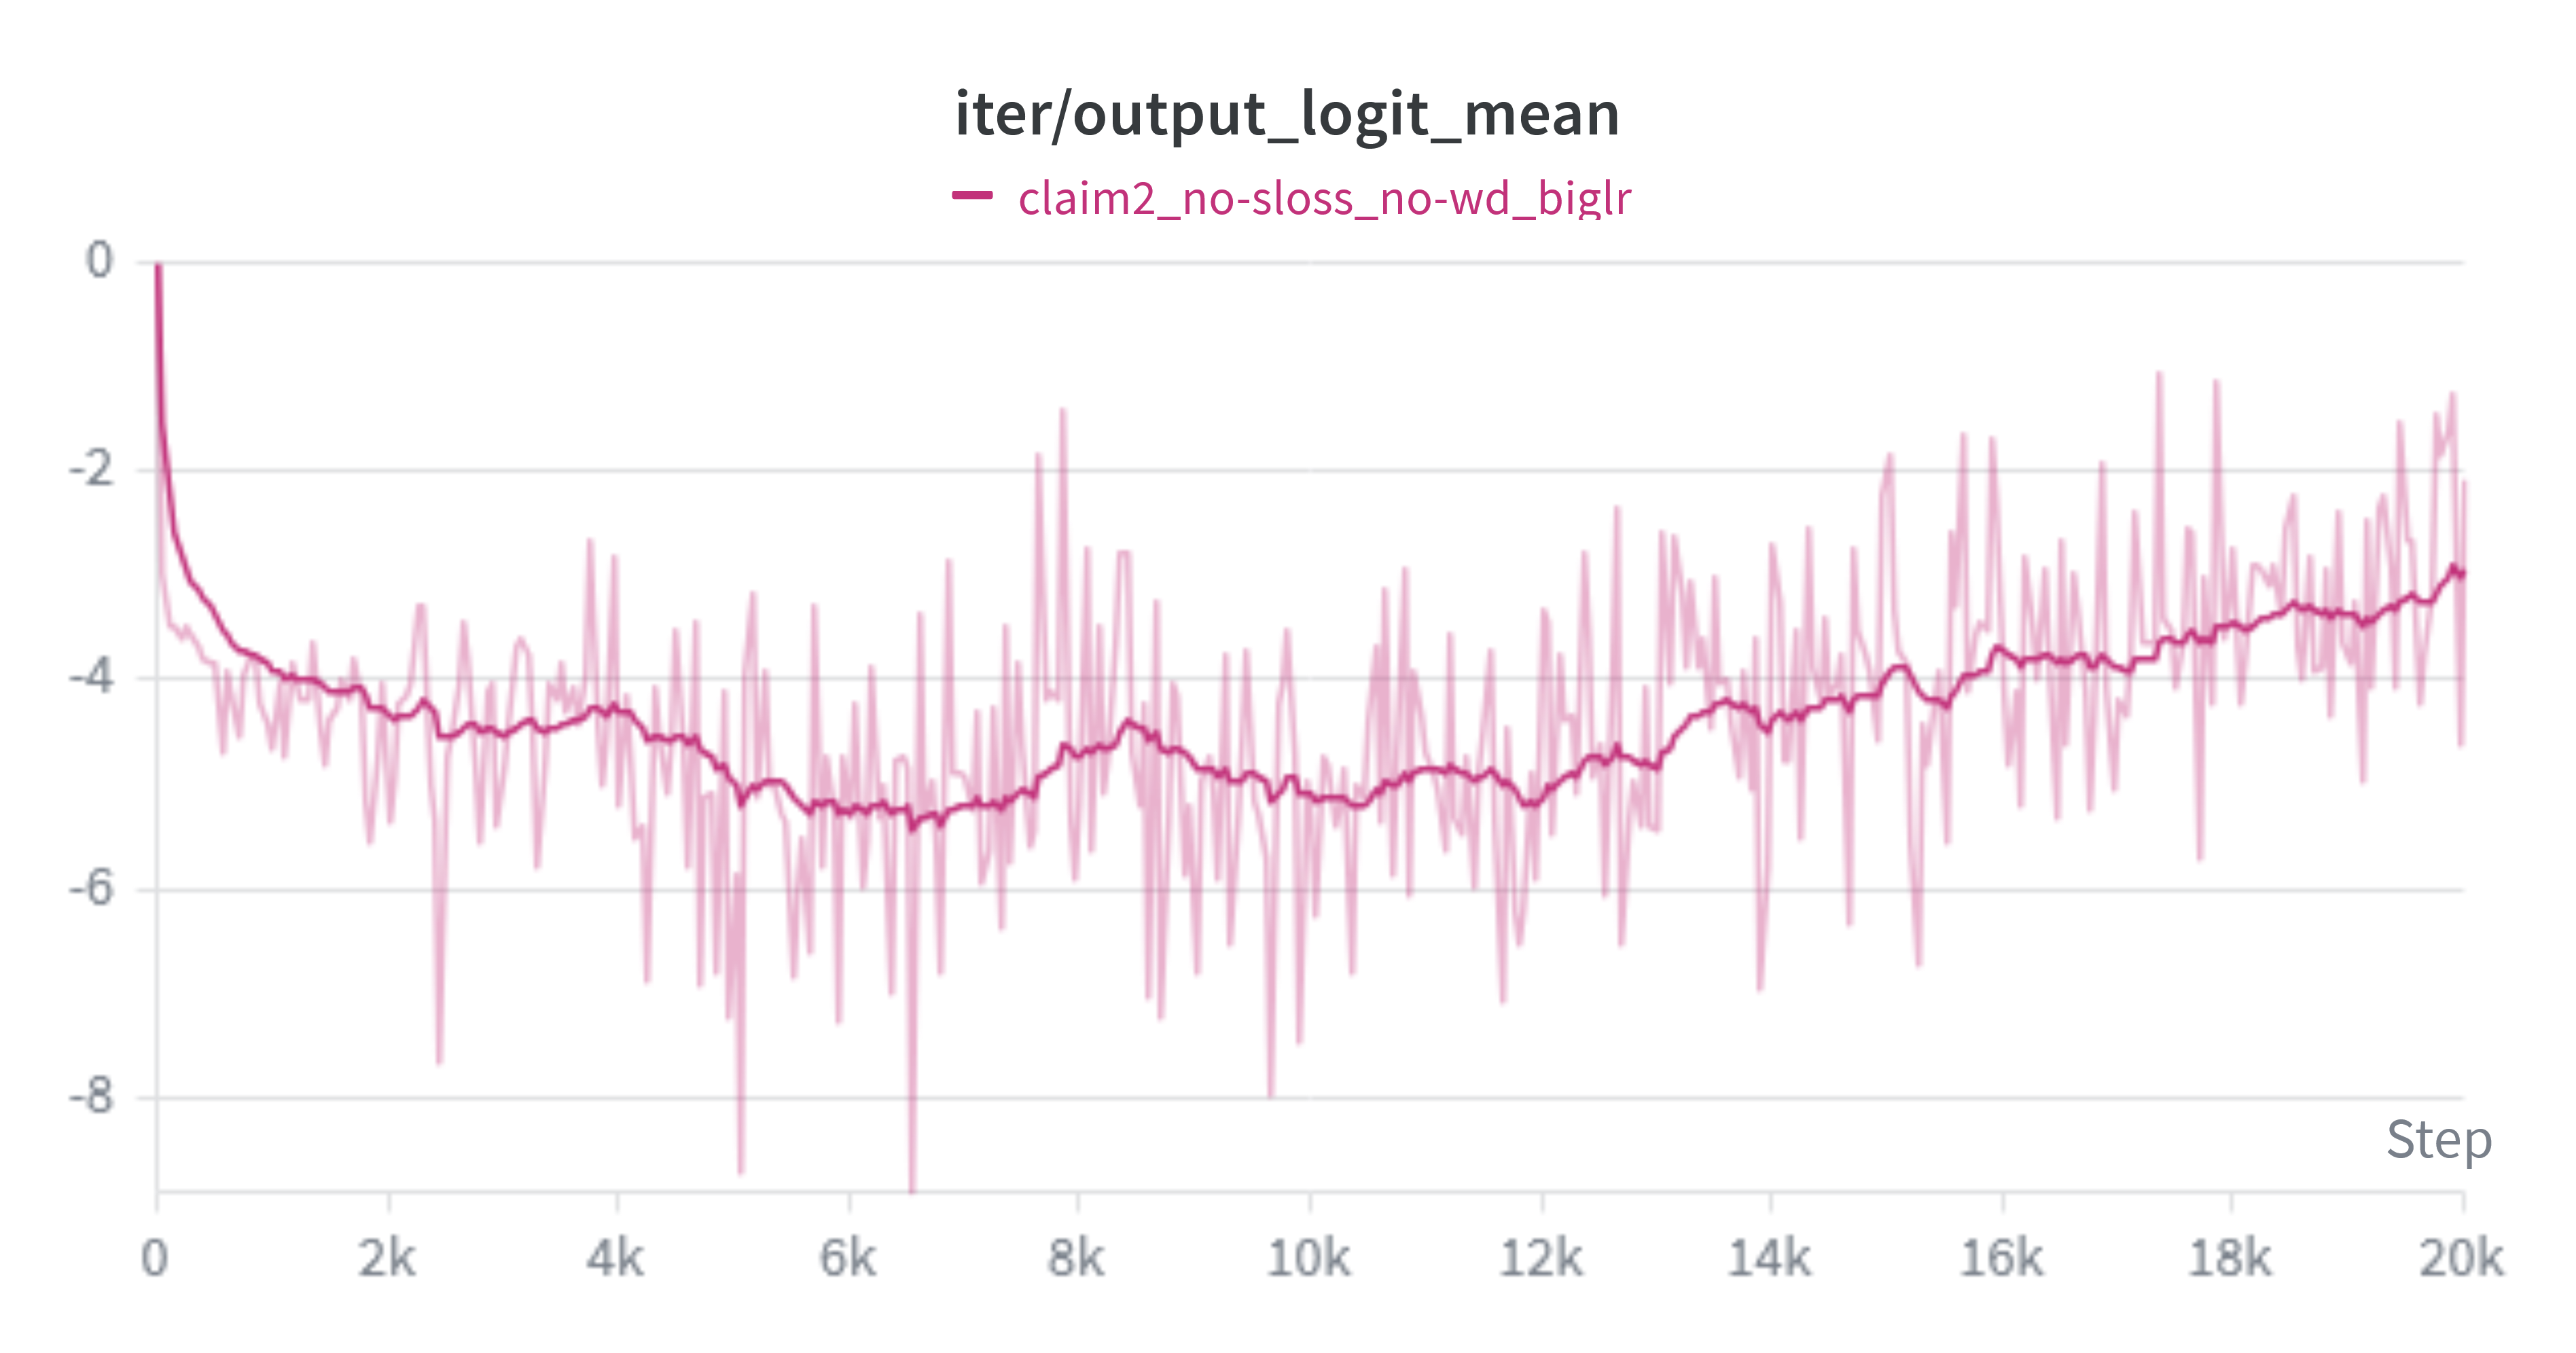
\includegraphics[width=\linewidth]{figures/C2_mean_meh_stable.png}
        \caption{Moderately stable — logit mean}
    \end{subfigure}

    \vspace{0.5em}

    % -------- Row 3: Unstable --------
    \begin{subfigure}{0.48\textwidth}
        \centering
        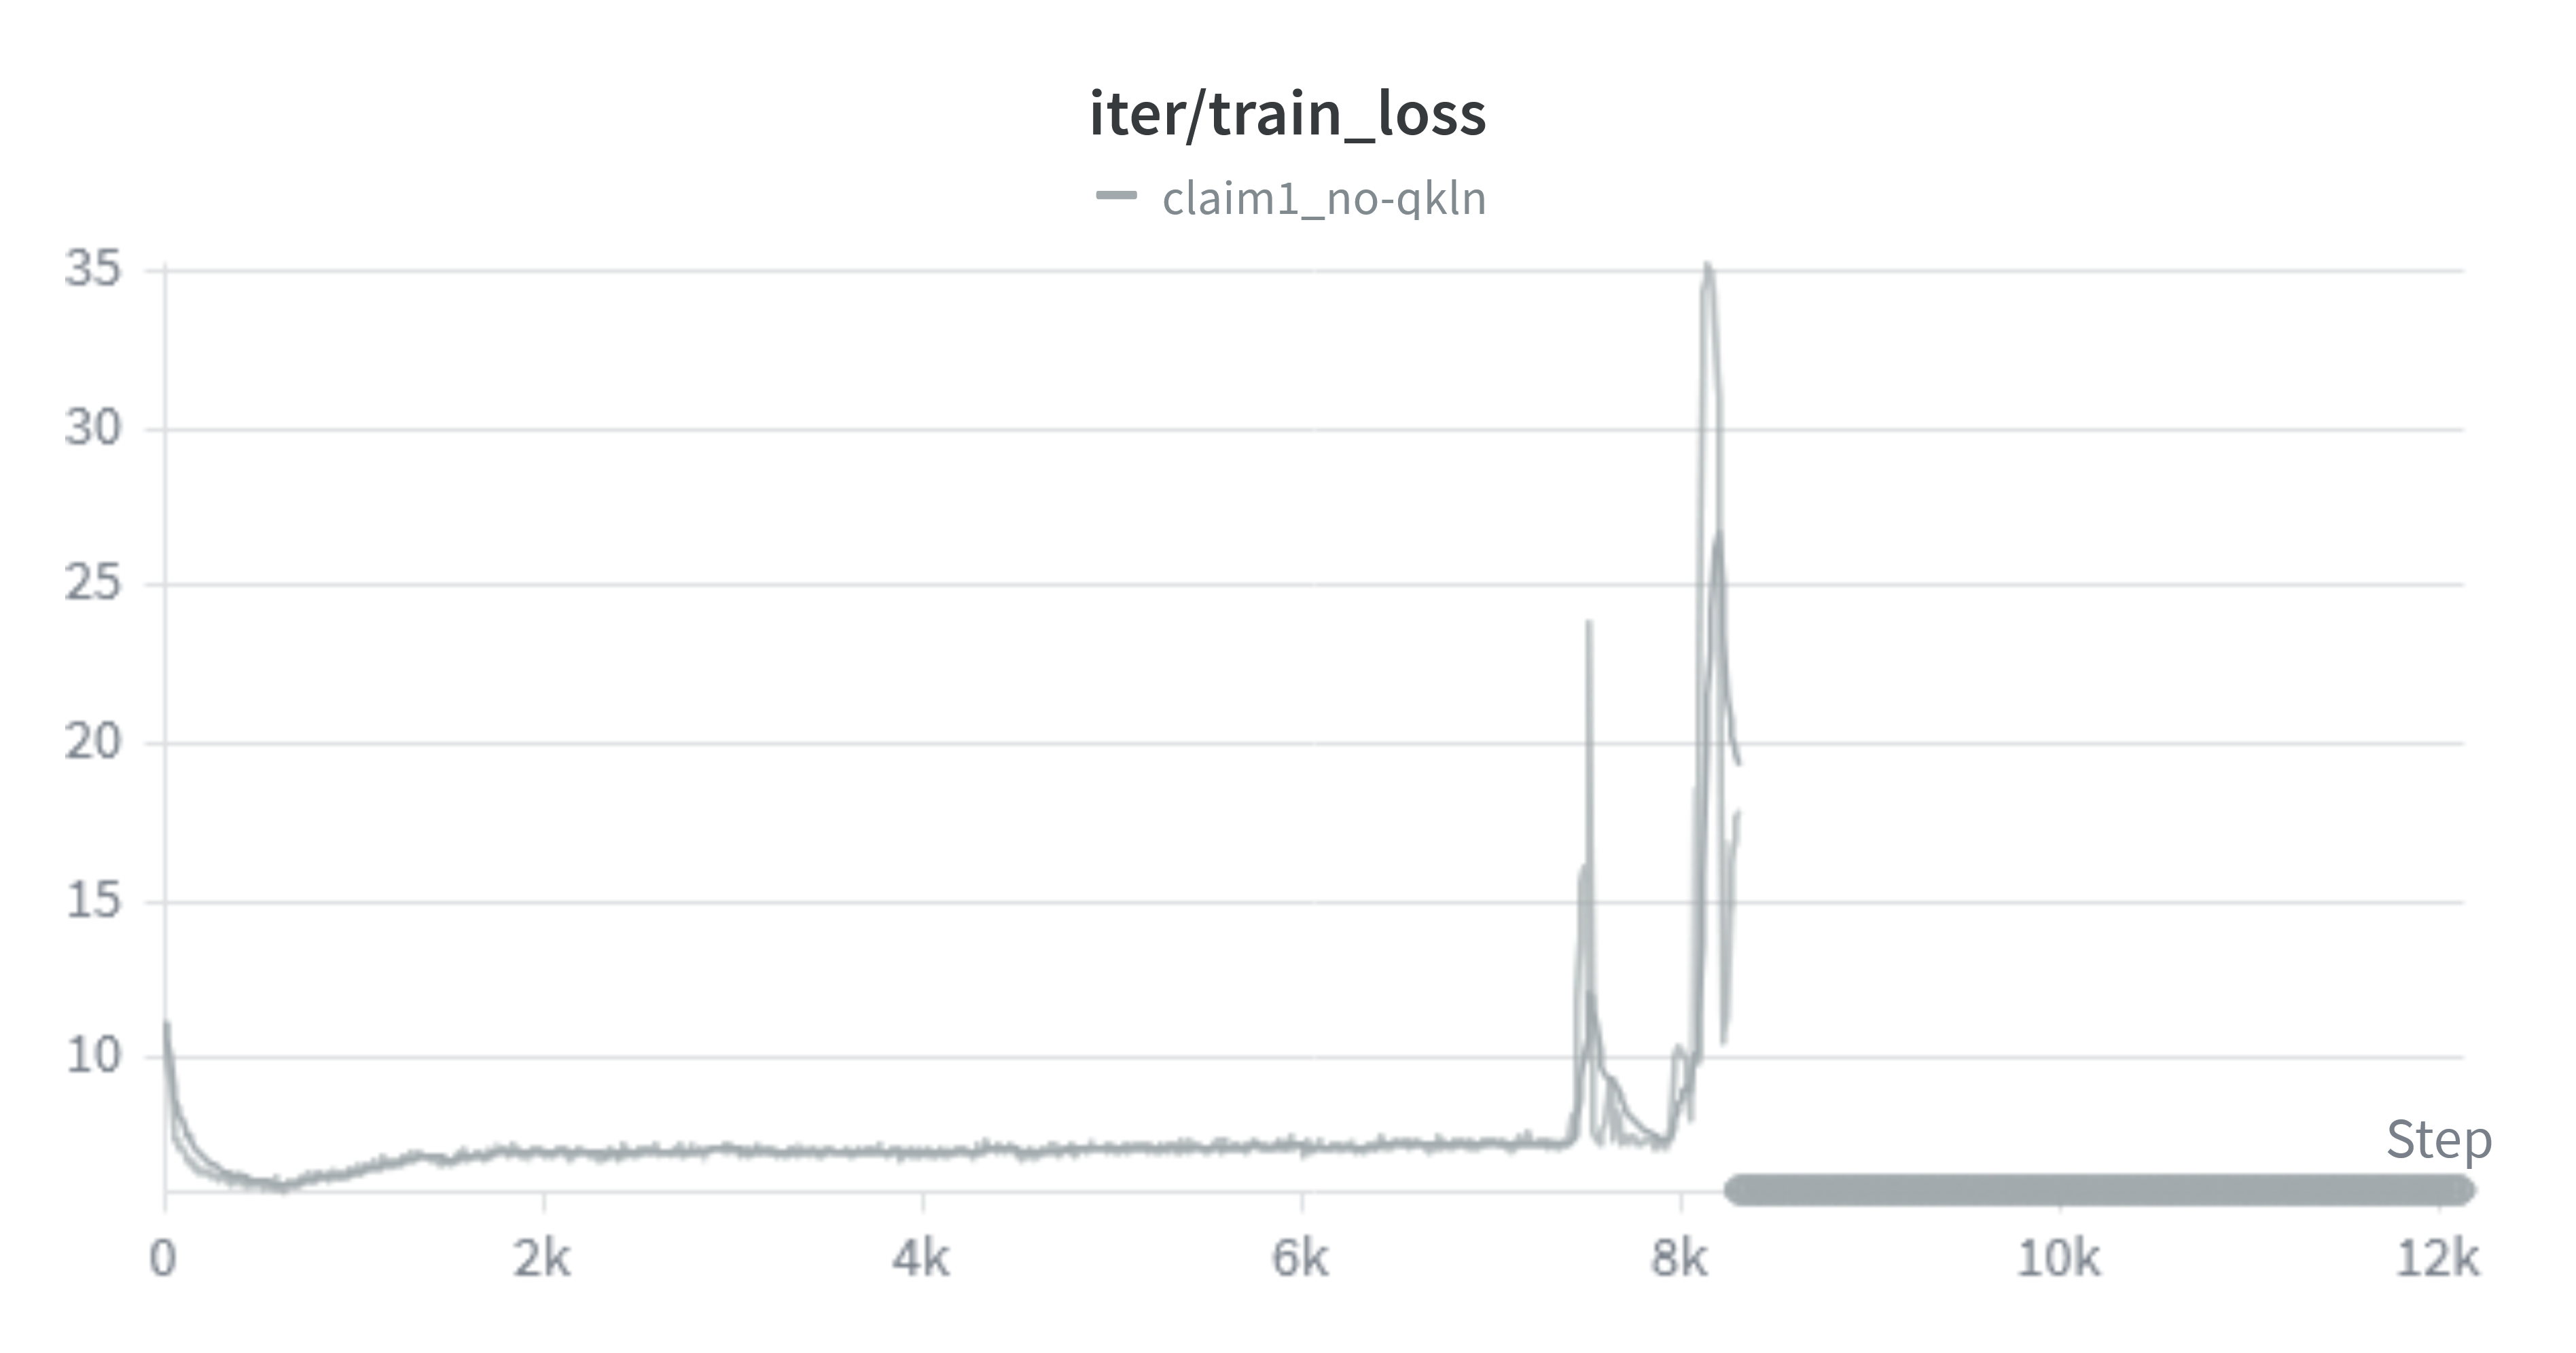
\includegraphics[width=\linewidth]{figures/C2_train_unstable.png}
        \caption{Unstable — train loss}
    \end{subfigure}
    \hfill
    \begin{subfigure}{0.48\textwidth}
        \centering
        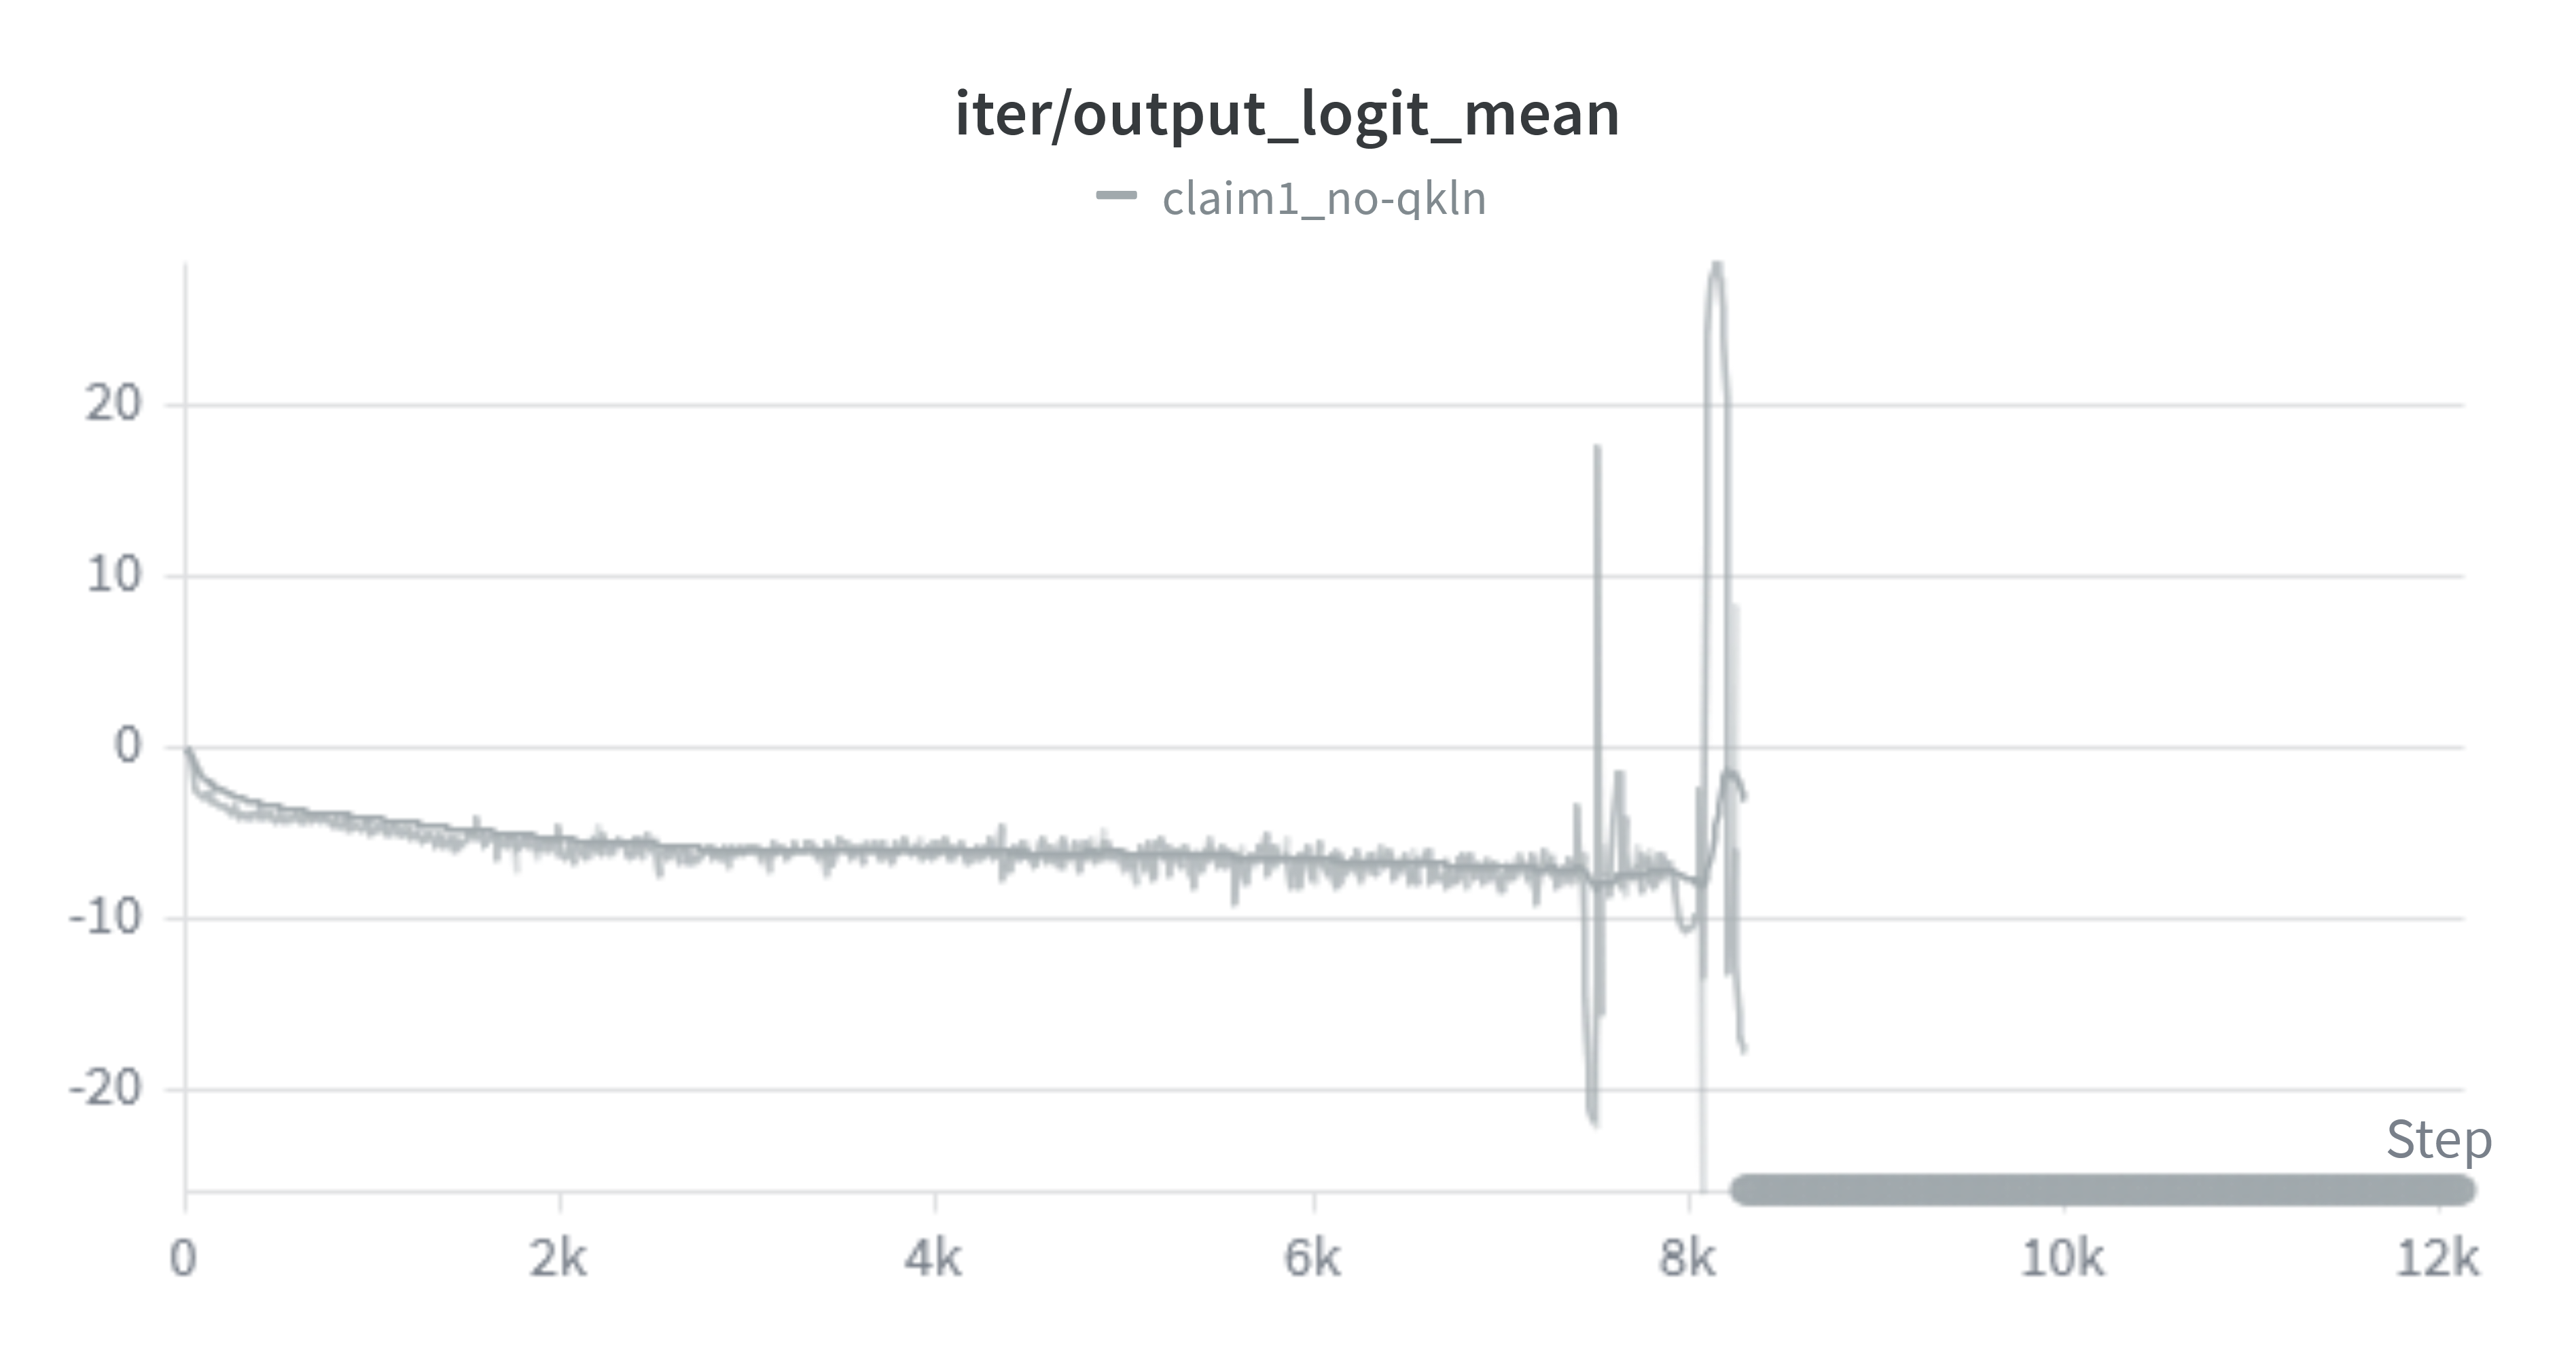
\includegraphics[width=\linewidth]{figures/C2_mean_unstable.png}
        \caption{Unstable — logit mean}
    \end{subfigure}

    \caption{Claim 2 experiments across three regimes. Top: stable training run(lr=0.1). Middle: moderately stable regime with mild fluctuations(lr linear warmup to 0.5). Bottom: unstable regime showing divergence. In three cases we did not observe a collapse to $-\infty$}
    \label{fig:claim2_grid}
\end{figure}
\paragraph{Takeaway.}
Our experiments therefore remain inconclusive for Claim~2.
They suggest that reproducing output-logit divergence may be more sensitive to
implementation details, model scale, or optimisation choices than suggested by
the simplified small-scale protocol alone.

% \input{sections/06_discussion}
% \input{sections/07_conclusion}

% ## Bibliography #############################################################
\bibliographystyle{abbrvnat}
\bibliography{references}

\end{document}